\documentclass{beamer}
\usepackage{graphicx}
\usepackage{bm}
\usepackage{xcolor}
\usepackage[ruled]{algorithm}
\usepackage{algorithmicx}
\usepackage[noend]{algpseudocode}
\usepackage{amsmath}
\usepackage{amssymb}
\usepackage{subcaption}
\usepackage{adjustbox}

\begin{document}
\beamertemplatenavigationsymbolsempty

\title{Temporal Smoothing in 2D Human Pose Estimation for Bouldering}

\author{André Oskar Andersen
\newline \small \texttt{wpr684}}

\institute{Institution of Computer Science, University of Copenhagen}

\date{2023}

\newcommand\unfootnote[1]{%
  \begingroup
  \renewcommand\thefootnote{}\footnote{#1}%
  \addtocounter{footnote}{-1}%
  \endgroup
}

\frame{\titlepage}

\begin{frame}
    \frametitle{Introduction}
    \begin{minipage}{0.5\textwidth}
        \begin{itemize}
            \item<1-> Increased usage of video analysis in sports.
            \begin{itemize}
                \item Help referee
                \item Improve techniques
            \end{itemize}
        \end{itemize}
    \end{minipage} \hfill
    \begin{minipage}{0.45\textwidth}
        \begin{figure}
            \center
            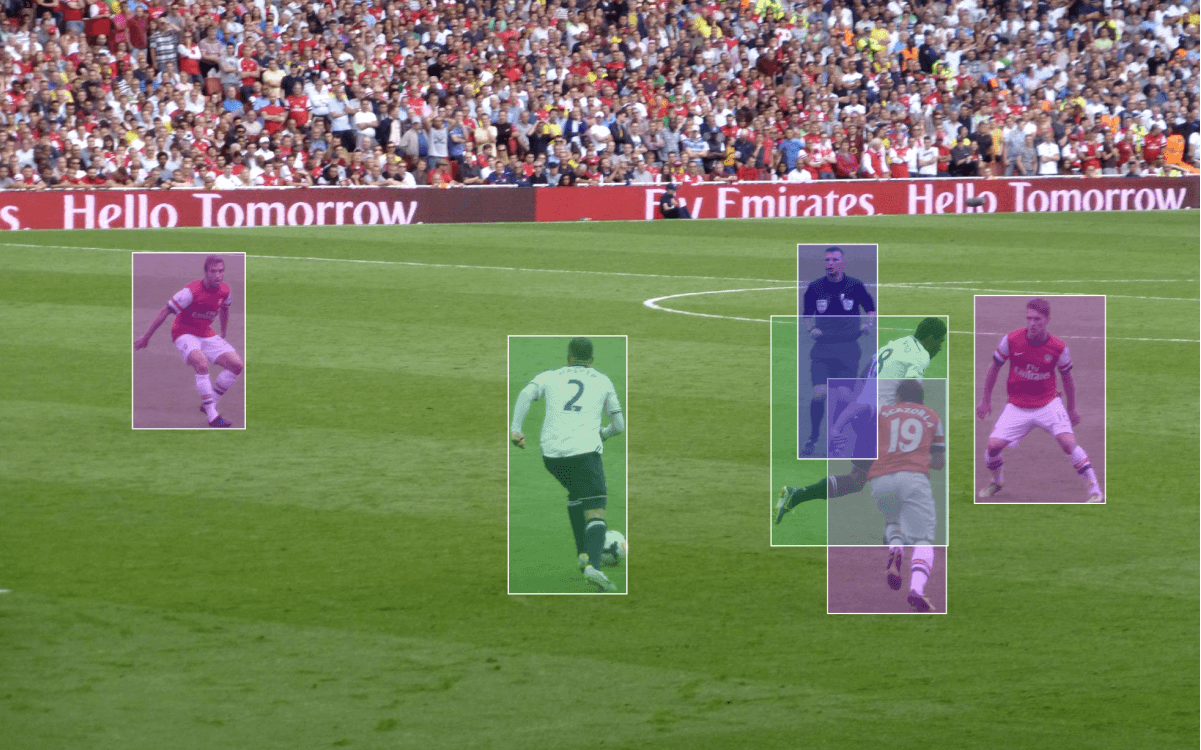
\includegraphics[width = \textwidth]{./entities/soccer_cv.png}
        \end{figure}
    \end{minipage}
    \unfootnote{\tiny \url{https://www.superannotate.com/blog/computer-vision-in-sports}}
\end{frame}

\begin{frame}
    \frametitle{Introduction}
    \begin{minipage}{0.5\textwidth}
        \begin{itemize}
            \item<1-> Increased usage of video analysis in sports.
            \item<1-> Often requires the position of the players.
            \begin{itemize}
                \item Already developed for popular sports.
                \item Missing for the less popular sports.
            \end{itemize}
        \end{itemize}
    \end{minipage} \hfill
    \begin{minipage}{0.45\textwidth}
        \begin{figure}
            \center
            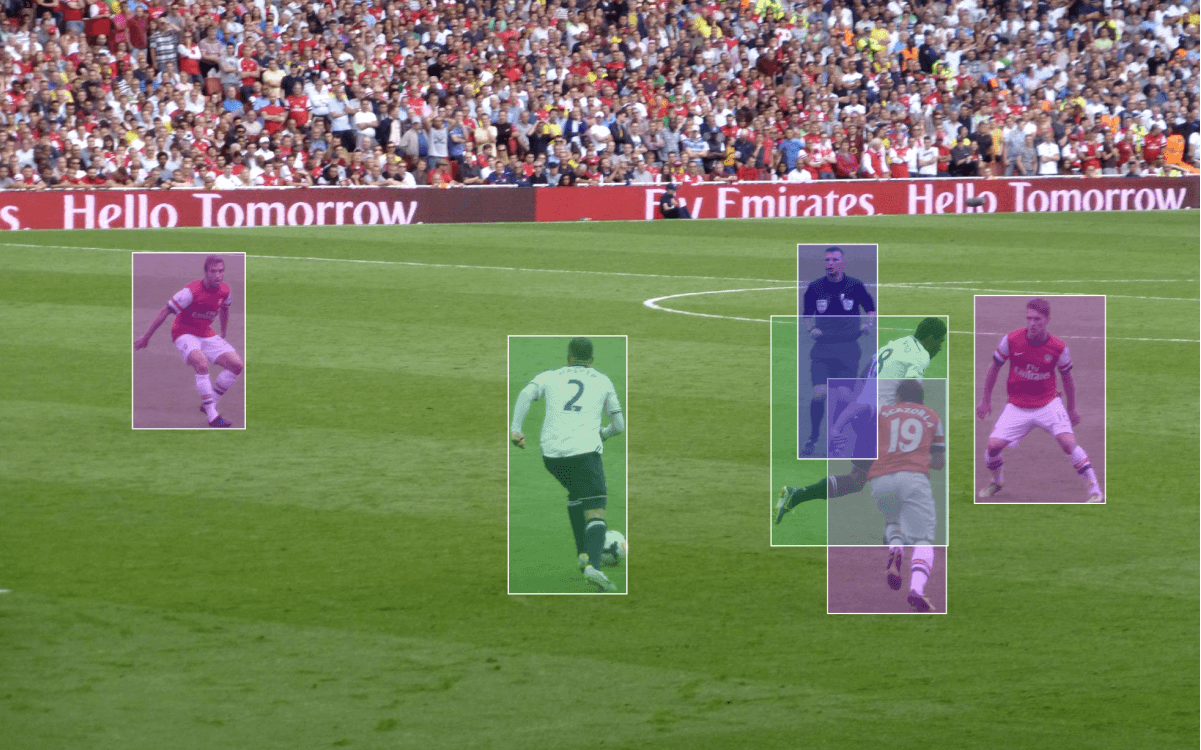
\includegraphics[width = \textwidth]{./entities/soccer_cv.png}
        \end{figure}
    \end{minipage}
    \unfootnote{\tiny \url{https://www.superannotate.com/blog/computer-vision-in-sports}}
\end{frame}

\begin{frame}
    \frametitle{Introduction}
    \begin{minipage}{0.5\textwidth}
        \begin{itemize}
            \item<1-> Increased usage of video analysis in sports.
            \item<1-> Often requires the position of the players.
            \item<1-> Problems with the data
            \begin{itemize}
                \item Methods require a lot of data
                \item Unusual poses/movements
            \end{itemize}
        \end{itemize}
    \end{minipage} \hfill
    \begin{minipage}{0.45\textwidth}
        \begin{figure}
            \center
            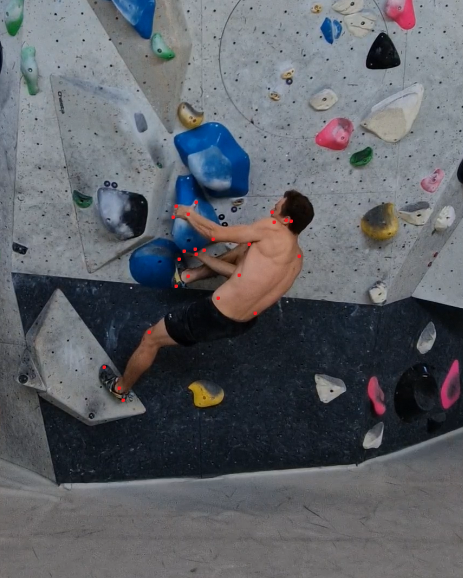
\includegraphics[width = \textwidth]{./entities/ClimbAlong_cv_2.PNG}
        \end{figure}
    \end{minipage}
    \unfootnote{\tiny \url{https://climbalong.com/lab}}
\end{frame}

\begin{frame}
    \frametitle{Introduction}
    \begin{minipage}{0.5\textwidth}
        \begin{itemize}
            \item<1-> Increased usage of video analysis in sports.
            \item<1-> Often requires the position of the players.
            \item<1-> Problems with the data
            \item<1-> ClimbAlong at NorthTech ApS
            \begin{itemize}
                \item<1-> Frame-independent pose-detector for bouldering - suboptimal results
                \item<2-> Proposition: Incorporate temporal information
            \end{itemize}
        \end{itemize}
    \end{minipage} \hfill
    \begin{minipage}{0.45\textwidth}
        \begin{figure}
            \center
            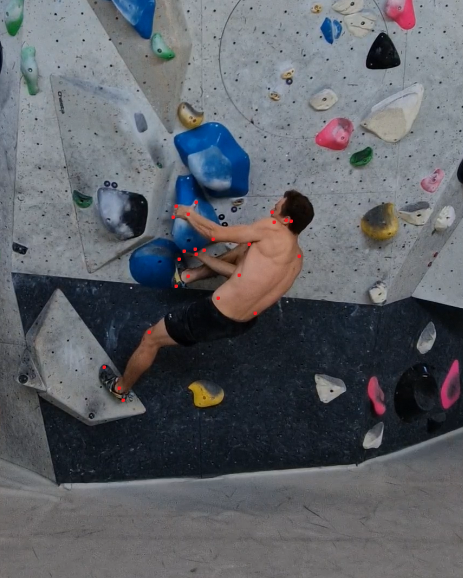
\includegraphics[width = \textwidth]{./entities/ClimbAlong_cv_2.PNG}
        \end{figure}
    \end{minipage}
    \unfootnote{\tiny \url{https://climbalong.com/lab}}
\end{frame}

\begin{frame}
    \frametitle{Introduction}
    \begin{itemize}
        \item<1-> Aim: extend the ClimbAlong pose-detector to use temporal information.
    \end{itemize}
\end{frame}

\begin{frame}
    \frametitle{The Models}
    \begin{itemize}
        \item<1-> Generally, three approaches
        \begin{enumerate}
            \item Convolutional layer
            \item Recurrent neural network (RNN)
            \item Transformer
        \end{enumerate}
        \item<2-> One of each approach
    \end{itemize}
    
\end{frame}

\begin{frame}
    \frametitle{The Models}
    Convolutional layer
    \begin{itemize}
        \item<1-> Name: 3DConv
        \item<1-> 3-dimensional conv. layer + ReLU
    \end{itemize}
    \begin{figure}
        \centering
        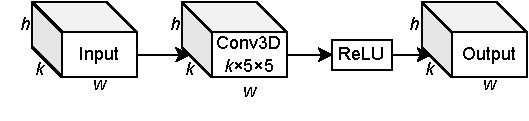
\includegraphics[width = 0.8\textwidth]{../report/entities/baseline.pdf}
    \end{figure}
\end{frame}

\begin{frame}
    \frametitle{The Models}
    RNN-based 1:
    \begin{itemize}
        \item<1-> Name: bi-ConvLSTM Model S
        \item<1-> Adaptation of Unipose-LSTM by Artacho and Savakis
        \item<1-> Bidirectional convolutional LSTM + 2D-conv. layers and ReLUs
        \item<1-> Processing directions summed together
    \end{itemize}
    \begin{figure}
        \centering
        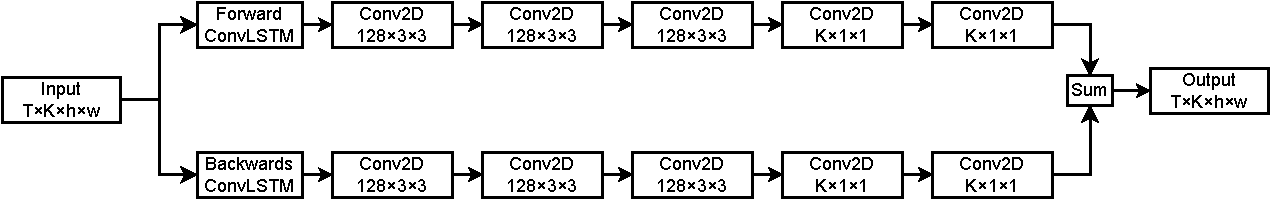
\includegraphics[width = \textwidth]{../report/entities/bi_conv_lstm.pdf}
    \end{figure}
    \unfootnote{\tiny \url{https://openaccess.thecvf.com/content_CVPR_2020/papers/Artacho_UniPose_Unified_Human_Pose_Estimation_in_Single_Images_and_Videos_CVPR_2020_paper.pdf}}
\end{frame}

\begin{frame}
    \frametitle{The Models}
    RNN-based 2:
    \begin{itemize}
        \item<1-> bi-ConvLSTM Model C
        \item<1-> Problem: Prioritization of processing direction
        \item<1-> Solution: Using convolution
        \item<1-> Otherwise, very similar to bi-ConvLSTM Model S
    \end{itemize}
    \begin{figure}
        \centering
        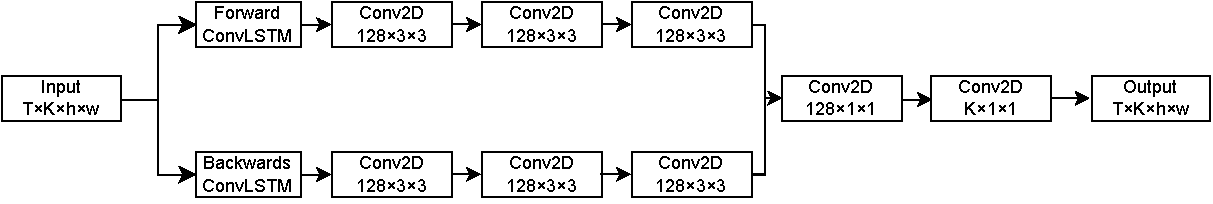
\includegraphics[width = \textwidth]{../report/entities/unipose2.pdf}
    \end{figure}
\end{frame}

\begin{frame}
    \frametitle{The Models}
    DeciWatch by Zeng \textit{Et al}.
    \begin{itemize}
        \item<1-> Transformer-based
        \item<1-> Samples every $n$th frame
        \item<1-> DenoiseNet + RecoverNet
    \end{itemize}
    \begin{figure}
        \centering
        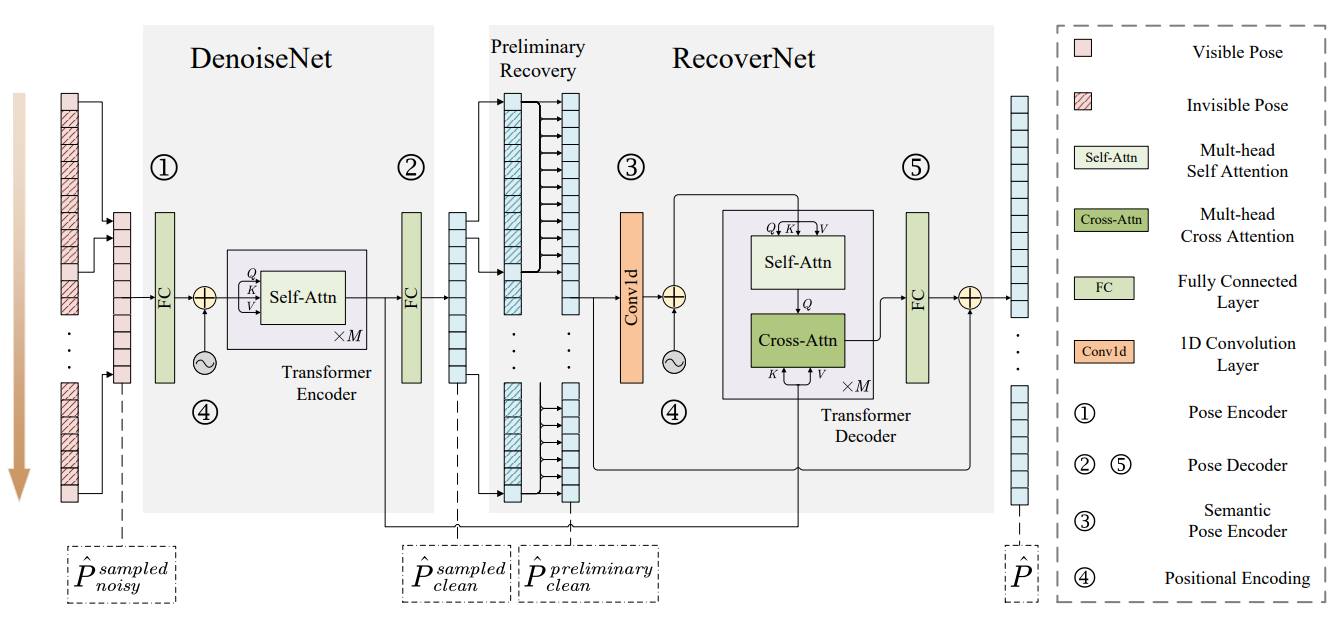
\includegraphics[width = \textwidth]{../report/entities/deciwatch.PNG}
    \end{figure}
    \unfootnote{\tiny \url{https://arxiv.org/pdf/2203.08713.pdf}}
\end{frame}

\begin{frame}
    \frametitle{The Data}
    \begin{minipage}{0.5\textwidth}
        ClimbAlong
        \begin{itemize}
            \item Fully annotated videos of climbers
            \item<2-> Problem: very small dataset
        \end{itemize}
    \end{minipage} \hfill
    \begin{minipage}{0.45\textwidth}
        \begin{figure}
            \center
            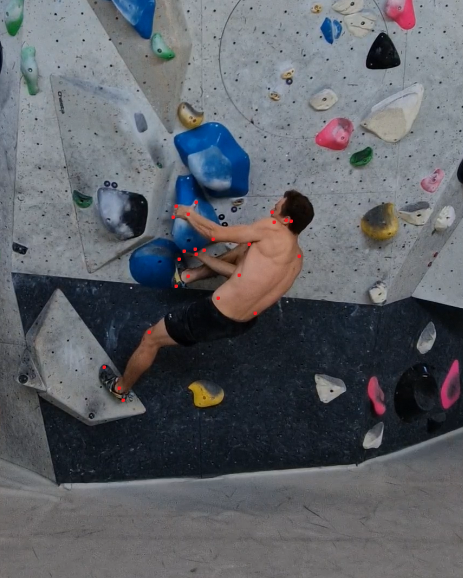
\includegraphics[width = \textwidth]{./entities/ClimbAlong_cv_2.PNG}
        \end{figure}
    \end{minipage}
    \unfootnote{\tiny \url{https://climbalong.com/lab}}
\end{frame}

\begin{frame}
    \frametitle{The Data}
    \begin{minipage}{0.5\textwidth}
        ClimbAlong
        \begin{itemize}
            \item Fully annotated videos of climbers
            \item Problem: Very small dataset
            \item Solution: pretrain on related datasets and finetune on ClimbAlong
            \begin{itemize}
                \item BRACE
                \item Penn Action
            \end{itemize}
        \end{itemize}
    \end{minipage} \hfill
    \begin{minipage}{0.45\textwidth}
        \begin{figure}
            \center
            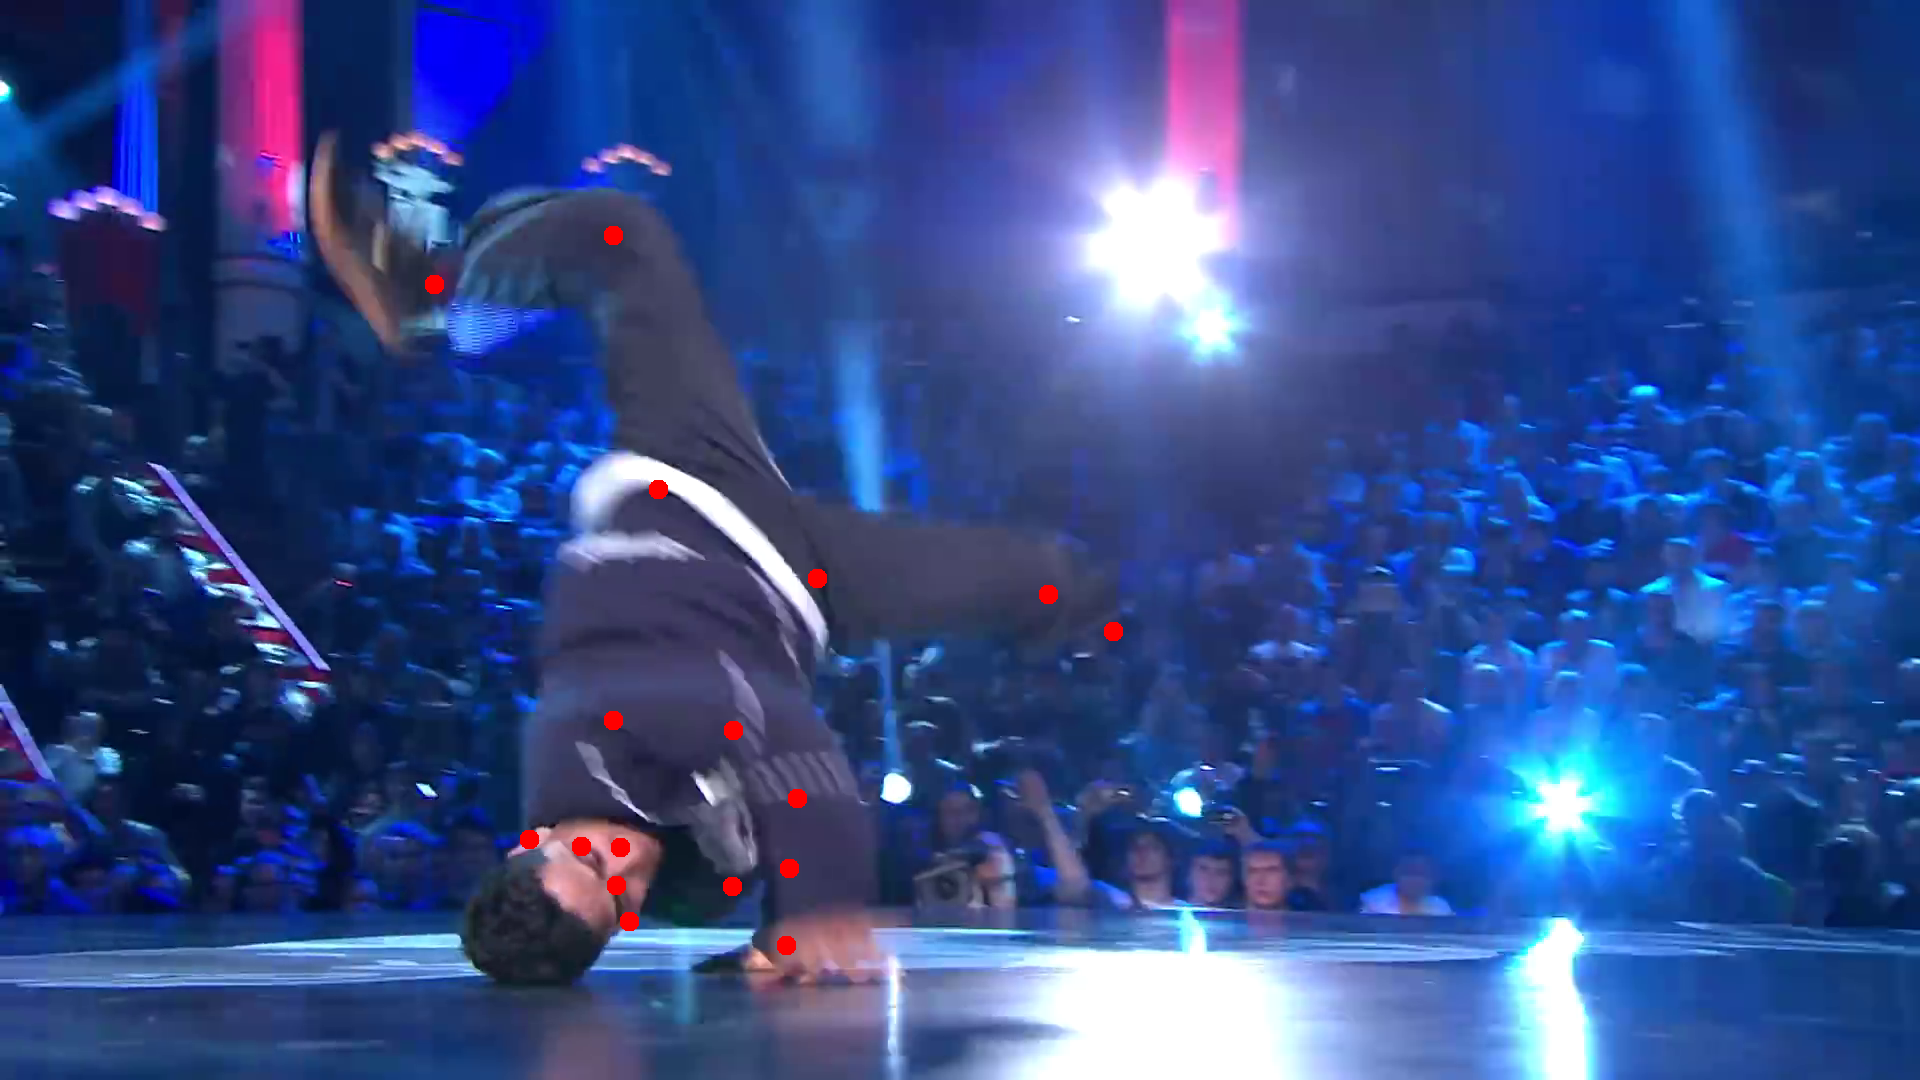
\includegraphics[width = \textwidth]{../report/entities/BRACE_1152.png}
            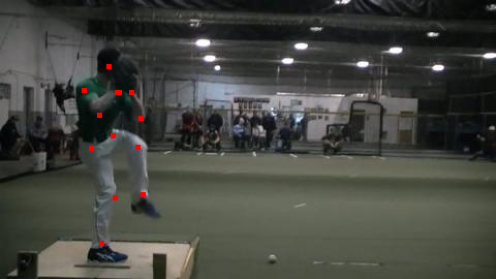
\includegraphics[width = \textwidth]{../report/entities/PA_64.png}
        \end{figure}
    \end{minipage}
\end{frame}

\begin{frame}
    \frametitle{Data Configuration}
    \begin{itemize}
        \item<1-> $s = 5$ frames, as 
        \begin{enumerate}
            \item<1-> Suggested by Artacho \textit{Et al.}
            \item<1-> Less memory
            \item<1-> Model-hyperparameter based on video length
        \end{enumerate}
        \item<2-> Creation of heatmaps
    \end{itemize}

    \only<2->{
        \begin{figure}
            \centering
            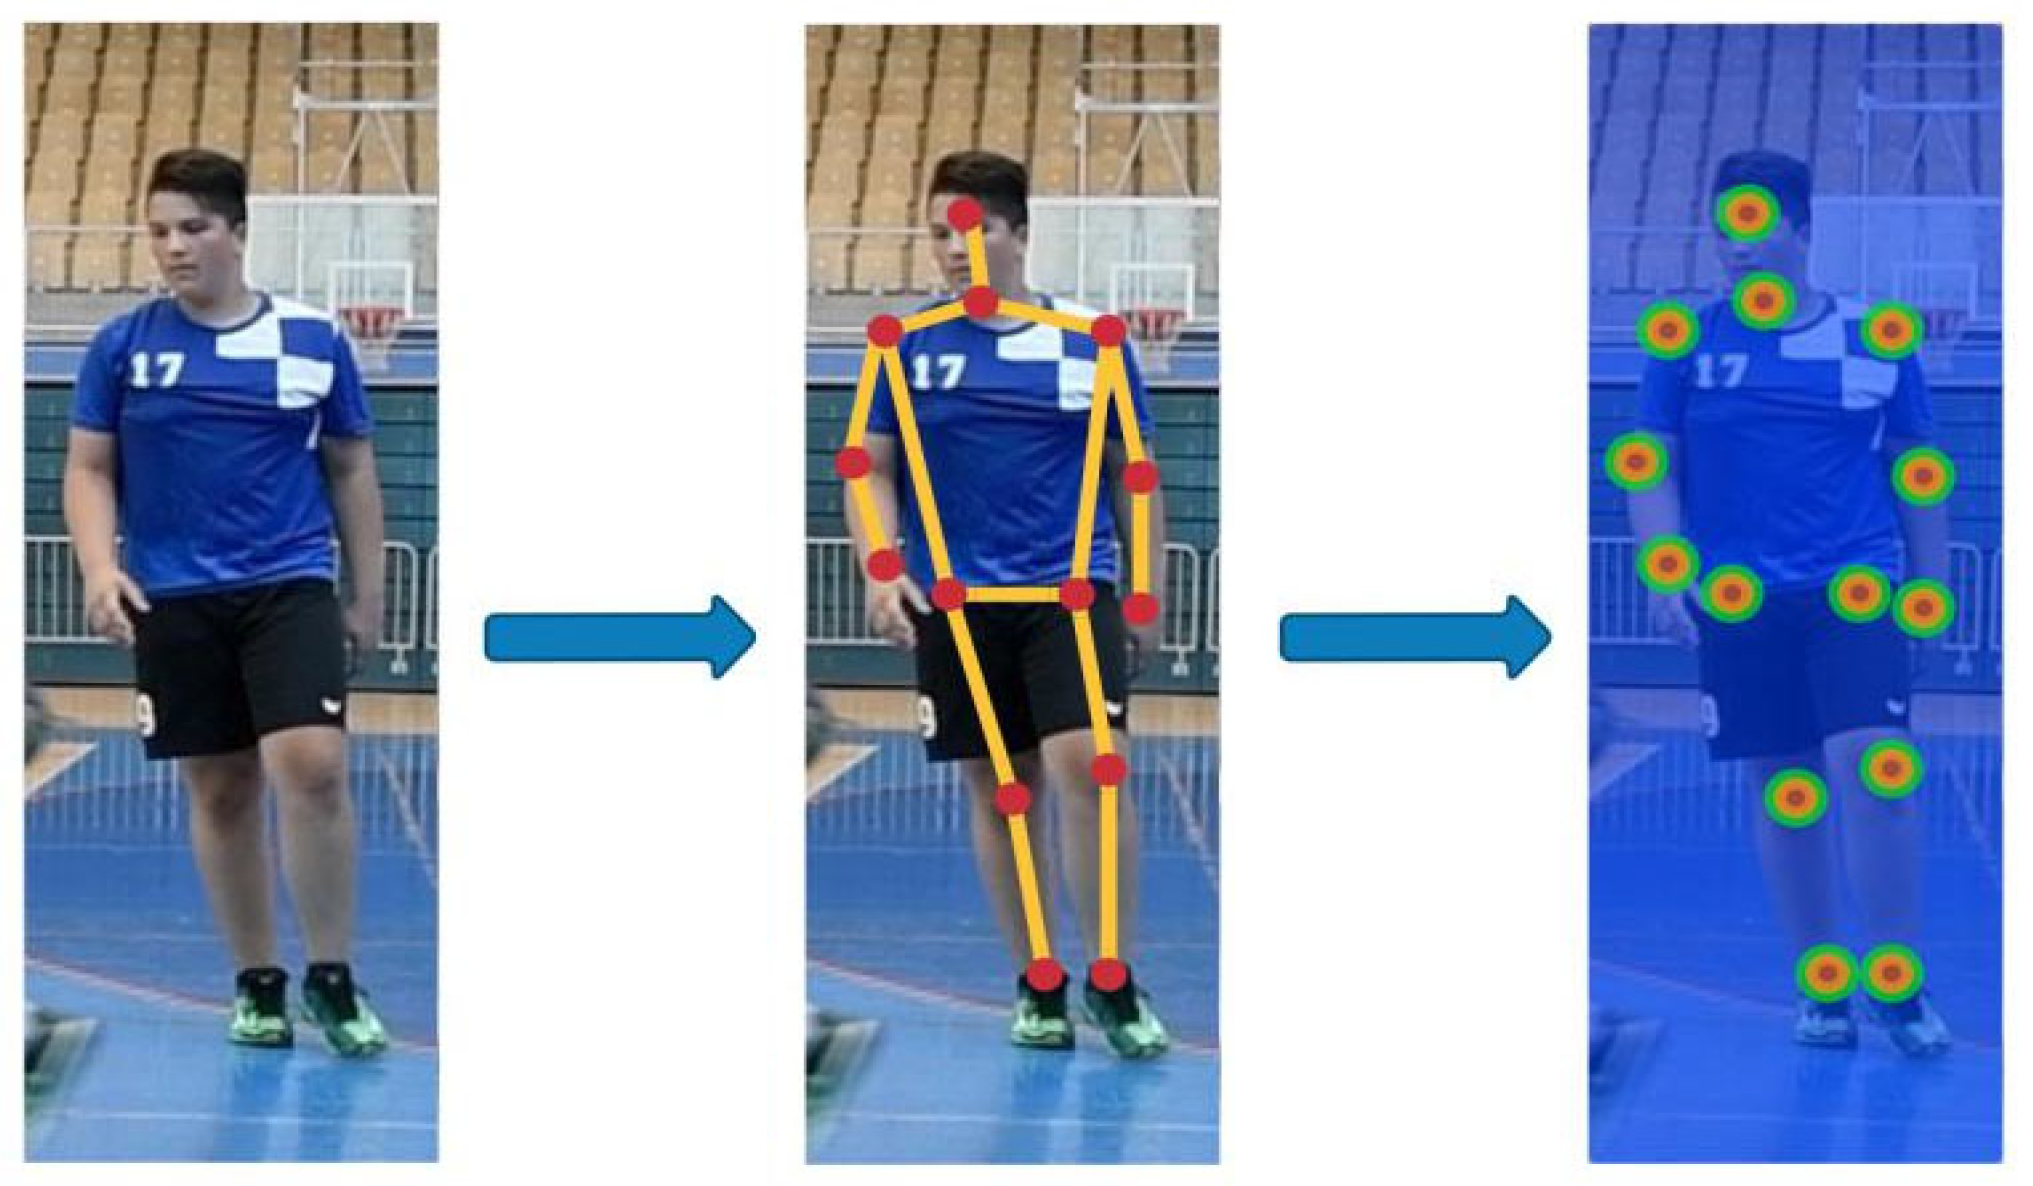
\includegraphics[width = 0.7 \textwidth]{./entities/heatmaps.png}
        \end{figure}
        \unfootnote{\tiny \url{https://www.mdpi.com/2313-433X/8/11/308}}
    }
    
    \unfootnote{\tiny https://arxiv.org/pdf/2001.08095.pdf}
\end{frame}

\begin{frame}
    \frametitle{Pretraining}
    Procedure
    \begin{itemize}
        \item<1-> Not training already-developed pose-detector
        \begin{itemize}
            \item Different input images = Bad representation of pose-detector predictions
        \end{itemize}
        \item<2-> Instead, simulate pose-detector output by shifting input keypoints = learn to denoise
    \end{itemize}
\end{frame}

\begin{frame}
    \frametitle{Pretraining}
    Finding optimal setting of models
    \begin{itemize}
        \item<1-> Three experiments
        \begin{enumerate}
            \item<1-> Various smearing standard deviations: pose-detector does not use fixed standard deviation
            \item<2-> Fixed smearing standard deviation: removed some of randomness from experiment 1
            \item<3-> Various smearing standard deviations + decreased frame rate: increased context
        \end{enumerate}
        \item<4-> Two different shifting-scalars
    \end{itemize}
\end{frame}

\begin{frame}
    \frametitle{Finetuning}
    Freezing already-developed pose-detector
        \begin{enumerate}
            \item Quicker fitting
            \item Greater understanding of results  
        \end{enumerate}
\end{frame}

\begin{frame}
    \frametitle{Accuracy metric}
    PCK: percentage of correct keypoints
    \begin{itemize}
        \item Correct if $dist(pred, gt) \leq d$
        \item PCK$@0.05$, PCK$@0.1$ and PCK$@0.2$ 
    \end{itemize}
\end{frame}

\begin{frame}
    \frametitle{Test results}
    \only<2->{Only minor difference:}
    
    \begin{itemize}
        \item<2-> Shifting-scalar: shifting-scalar $s = 1$ better simulates the pose-detector
        \item<3-> Translation + scaling vs only translation: standard deviations of peaks in ClimbAlong data not changing as much
    \end{itemize}
    \begin{table}[htbp]
        \scalebox{0.7}{
            \begin{tabular}{c||ccc|ccc|ccc}
                \hline
                Accuracy metric & \multicolumn{3}{c}{PCK@0.05} & \multicolumn{3}{c}{PCK@0.1} & \multicolumn{3}{c}{PCK@0.2} \\
                \hline
                Experiment & 1 & 2 & 3 & 1 & 2 & 3 & 1 & 2 & 3 \\
                \hline
                \hline
                Identity function & 19.4 & 19.4 & 19.4 & 66.1 & 66.1 & 66.1 & 85.2 & 85.2 & 85.2 \\
                3DConv & 49.7 & 52.3 & 53.1 & 95.7 & 95.7 & 95.8 & 99.2 & 99.3 & 99.3 \\
                DeciWatch & 76.6 & 76.7 & 68.1 & 94.4 & 94.3 & 87.3 & 99.2 & 99.2 & 96.1 \\
                bi-ConvLSTM - Model S & 37.8 & 34.9 & 39.0 & 91.8 & 92.1 & 92.2 & 99.4 & 99.7 & 99.2 \\
                bi-ConvLSTM - Model C & 35.9 & 39.0 & 38.5 & 93.1 & 93.6 & 92.6 & 99.8 & 99.7 & 99.7 \\
                \hline
            \end{tabular}
        }
    \end{table}
    
    \begin{table}[htbp]
        \scalebox{0.7}{
            \begin{tabular}{c||ccc|ccc|ccc}
                \hline
                Accuracy metric & \multicolumn{3}{c}{PCK@0.05} & \multicolumn{3}{c}{PCK@0.1} & \multicolumn{3}{c}{PCK@0.2} \\
                \hline
                Experiment & 1 & 2 & 3 & 1 & 2 & 3 & 1 & 2 & 3 \\
                \hline
                \hline
                Identity function & 19.4 & 19.4 & 19.4 & 66.1 & 66.1 & 66.1 & 85.2 & 85.2 & 85.2 \\
                3DConv & 46.5 & 51.6 & 47.3 & 95.5 & 95.5 & 95.8 & 99.2 & 99.3 & 99.2 \\
                DeciWatch & 76.0 & 75.9 & 36.8 & 94.2 & 94.2 & 74.9 & 99.2 & 99.2 & 92.8 \\
                bi-ConvLSTM - Model S & 38.8 & 37.4 & 35.9 & 92.7 & 92.1 & 91.2 & 99.4 & 99.5 & 99.3 \\
                bi-ConvLSTM - Model C & 39.2 & 39.5 & 37.1 & 92.5 & 92.9 & 92.6 & 99.6 & 99.3 & 99.6 \\
                \hline
            \end{tabular}
        }
    \end{table}
\end{frame}


\begin{frame}
    \frametitle{Test results}
    Decreased frame rate:
    \begin{itemize}
        \item 3DConv: benefit
        \item DeciWatch: drawback
        \item bi-ConvLSTM: benefit for less noise
    \end{itemize}
    \begin{table}[htbp]
        \scalebox{0.7}{
            \begin{tabular}{c||ccc|ccc|ccc}
                \hline
                Accuracy metric & \multicolumn{3}{c}{PCK@0.05} & \multicolumn{3}{c}{PCK@0.1} & \multicolumn{3}{c}{PCK@0.2} \\
                \hline
                Experiment & 1 & 2 & 3 & 1 & 2 & 3 & 1 & 2 & 3 \\
                \hline
                \hline
                Identity function & 19.4 & 19.4 & 19.4 & 66.1 & 66.1 & 66.1 & 85.2 & 85.2 & 85.2 \\
                3DConv & 49.7 & 52.3 & 53.1 & 95.7 & 95.7 & 95.8 & 99.2 & 99.3 & 99.3 \\
                DeciWatch & 76.6 & 76.7 & 68.1 & 94.4 & 94.3 & 87.3 & 99.2 & 99.2 & 96.1 \\
                bi-ConvLSTM - Model S & 37.8 & 34.9 & 39.0 & 91.8 & 92.1 & 92.2 & 99.4 & 99.7 & 99.2 \\
                bi-ConvLSTM - Model C & 35.9 & 39.0 & 38.5 & 93.1 & 93.6 & 92.6 & 99.8 & 99.7 & 99.7 \\
                \hline
            \end{tabular}
        }
    \end{table}
    
    \begin{table}[htbp]
        \scalebox{0.7}{
            \begin{tabular}{c||ccc|ccc|ccc}
                \hline
                Accuracy metric & \multicolumn{3}{c}{PCK@0.05} & \multicolumn{3}{c}{PCK@0.1} & \multicolumn{3}{c}{PCK@0.2} \\
                \hline
                Experiment & 1 & 2 & 3 & 1 & 2 & 3 & 1 & 2 & 3 \\
                \hline
                \hline
                Identity function & 19.4 & 19.4 & 19.4 & 66.1 & 66.1 & 66.1 & 85.2 & 85.2 & 85.2 \\
                3DConv & 46.5 & 51.6 & 47.3 & 95.5 & 95.5 & 95.8 & 99.2 & 99.3 & 99.2 \\
                DeciWatch & 76.0 & 75.9 & 36.8 & 94.2 & 94.2 & 74.9 & 99.2 & 99.2 & 92.8 \\
                bi-ConvLSTM - Model S & 38.8 & 37.4 & 35.9 & 92.7 & 92.1 & 91.2 & 99.4 & 99.5 & 99.3 \\
                bi-ConvLSTM - Model C & 39.2 & 39.5 & 37.1 & 92.5 & 92.9 & 92.6 & 99.6 & 99.3 & 99.6 \\
                \hline
            \end{tabular}
        }
    \end{table}
\end{frame}

\begin{frame}
    \frametitle{Test results}
    bi-ConvLSTM: Model S vs Model C:
    \begin{itemize}
        \item Not as a big of a concern
    \end{itemize}
    \begin{table}[htbp]
        \scalebox{0.7}{
            \begin{tabular}{c||ccc|ccc|ccc}
                \hline
                Accuracy metric & \multicolumn{3}{c}{PCK@0.05} & \multicolumn{3}{c}{PCK@0.1} & \multicolumn{3}{c}{PCK@0.2} \\
                \hline
                Experiment & 1 & 2 & 3 & 1 & 2 & 3 & 1 & 2 & 3 \\
                \hline
                \hline
                Identity function & 19.4 & 19.4 & 19.4 & 66.1 & 66.1 & 66.1 & 85.2 & 85.2 & 85.2 \\
                3DConv & 49.7 & 52.3 & 53.1 & 95.7 & 95.7 & 95.8 & 99.2 & 99.3 & 99.3 \\
                DeciWatch & 76.6 & 76.7 & 68.1 & 94.4 & 94.3 & 87.3 & 99.2 & 99.2 & 96.1 \\
                bi-ConvLSTM - Model S & 37.8 & 34.9 & 39.0 & 91.8 & 92.1 & 92.2 & 99.4 & 99.7 & 99.2 \\
                bi-ConvLSTM - Model C & 35.9 & 39.0 & 38.5 & 93.1 & 93.6 & 92.6 & 99.8 & 99.7 & 99.7 \\
                \hline
            \end{tabular}
        }
    \end{table}
    
    \begin{table}[htbp]
        \scalebox{0.7}{
            \begin{tabular}{c||ccc|ccc|ccc}
                \hline
                Accuracy metric & \multicolumn{3}{c}{PCK@0.05} & \multicolumn{3}{c}{PCK@0.1} & \multicolumn{3}{c}{PCK@0.2} \\
                \hline
                Experiment & 1 & 2 & 3 & 1 & 2 & 3 & 1 & 2 & 3 \\
                \hline
                \hline
                Identity function & 19.4 & 19.4 & 19.4 & 66.1 & 66.1 & 66.1 & 85.2 & 85.2 & 85.2 \\
                3DConv & 46.5 & 51.6 & 47.3 & 95.5 & 95.5 & 95.8 & 99.2 & 99.3 & 99.2 \\
                DeciWatch & 76.0 & 75.9 & 36.8 & 94.2 & 94.2 & 74.9 & 99.2 & 99.2 & 92.8 \\
                bi-ConvLSTM - Model S & 38.8 & 37.4 & 35.9 & 92.7 & 92.1 & 91.2 & 99.4 & 99.5 & 99.3 \\
                bi-ConvLSTM - Model C & 39.2 & 39.5 & 37.1 & 92.5 & 92.9 & 92.6 & 99.6 & 99.3 & 99.6 \\
                \hline
            \end{tabular}
        }
    \end{table}
\end{frame}

\begin{frame}
    \frametitle{Test results}
    Worst performing keypoints:
    \begin{itemize}
        \item Pinkies, index fingers and thumbs
        \item Not included during pretraining (minor effect - heels and toes)
        \item A lot of movement
    \end{itemize}
    \begin{figure}
        \centering
        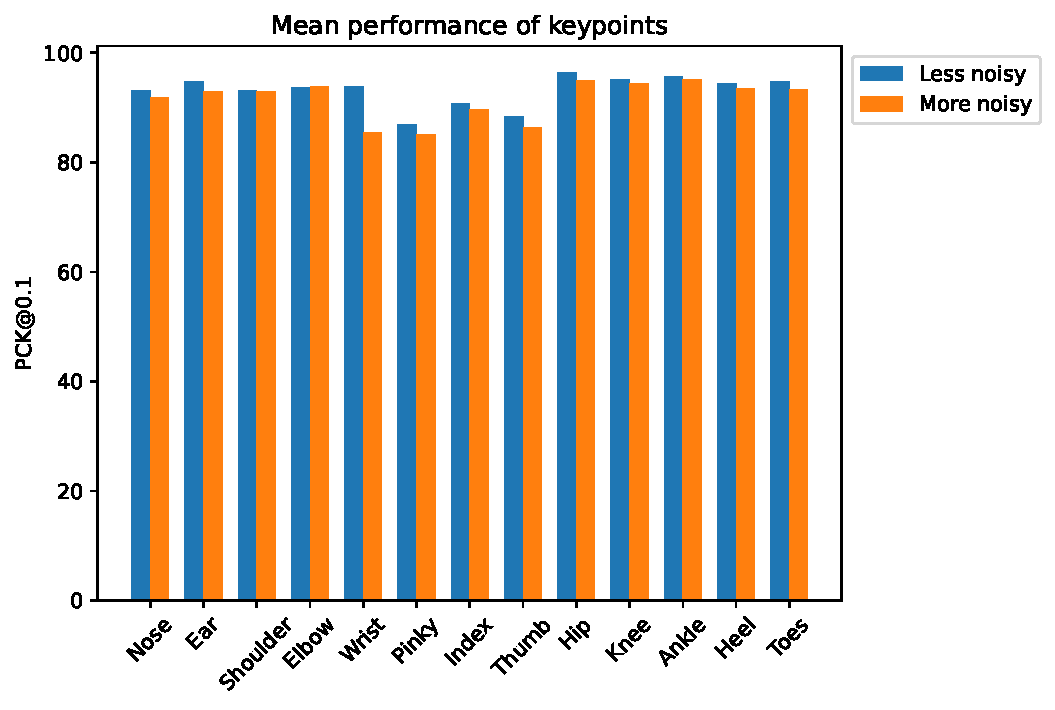
\includegraphics[width = 0.7\textwidth]{entities/kpts.pdf}
    \end{figure}
\end{frame}

\begin{frame}
    \frametitle{Test results}
    Worst performing keypoints:
    \begin{itemize}
        \item Pinkies, index fingers and thumbs
        \item Not included during pretraining (minor effect - heels and toes)
        \item A lot of movement
        \item Extra: performance of pose-detector
    \end{itemize}
    \begin{figure}
        \centering
        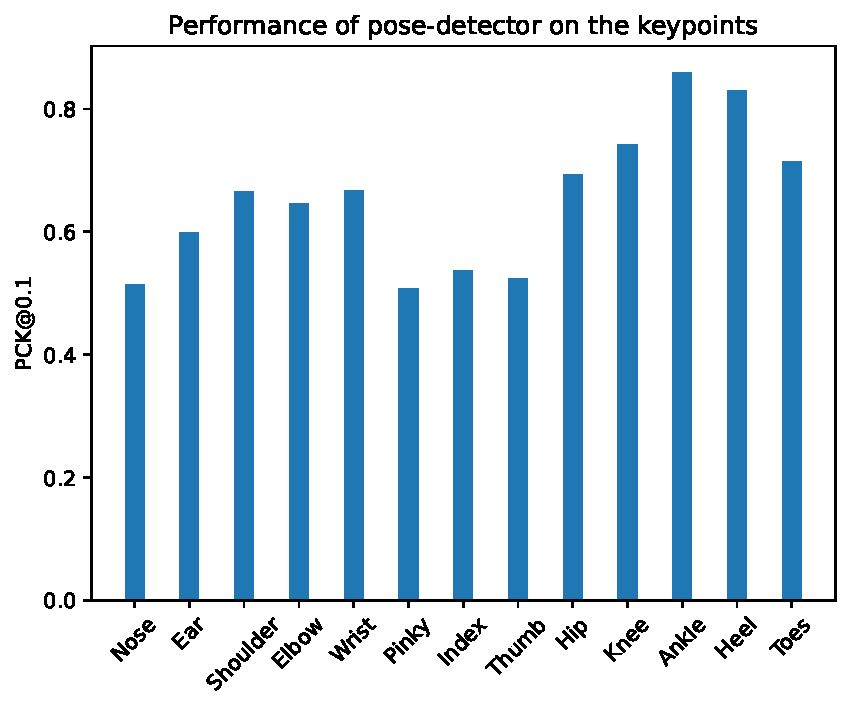
\includegraphics[width = 0.6\textwidth]{entities/kpts_pose_detector.pdf}
    \end{figure}
\end{frame}


\begin{frame}
    \frametitle{Which model is the optimal choice?}
    \begin{itemize}
        \item<1-> Greatest testing accuracy: DeciWatch shifting-scalar $s = 1$, full frame rate
        \item<1-> Greatest rough estimation: bi-ConvLSTM Model C, shifting-scalar $s = 1$, experiment 1
        \item<1-> Speed and memory: 3DConv, shfting-scalar $s = 1$, experiment 3
    \end{itemize}

    \only<1->{
        \begin{table}[htbp]
            \scalebox{0.7}{
                \centering
                \begin{tabular}{c||ccc}
                    \hline
                    & \begin{tabular}[c]{@{}c@{}}Mean\\prediction time (ms) \end{tabular} & \begin{tabular}[c]{@{}c@{}}Standard deviation\\of prediction time (ms)\end{tabular} & \begin{tabular}[c]{@{}c@{}}Number of\\parameters\end{tabular} \\
                    \hline
                    \hline 
                    3DConv & $0.39$ & $9.29 \times 10^{-2}$ & 78,150\\
                    DeciWatch & $14.2$ & $0.11$  & 1,708,388 \\
                    bi-ConvLSTM - Model S & $10.6$ & $1.68 \times 10^{-2}$ & 1,875,666 \\
                    bi-ConvLSTM - Model C & $20.1$ & $6.93 \times 10^{-2}$ & 1,872,313 \\
                    \hline
                \end{tabular}
            }
        \end{table}
    }
\end{frame}

\begin{frame}
    \frametitle{General reflections}
    Potential mistakes we have made
    \begin{itemize}
        \item<1-> Pretraining
        \begin{itemize}
            \item<1-> Should have estimated parameters of data
            \item<2-> Same video sequence across subsets = could carry some bias
        \end{itemize}
        \item<3-> Finetuning
        \begin{itemize}
            \item<3-> Groundtruth outside of bbox 
        \end{itemize}
    \end{itemize}
    \only<3>{
        \begin{figure}
            \centering
            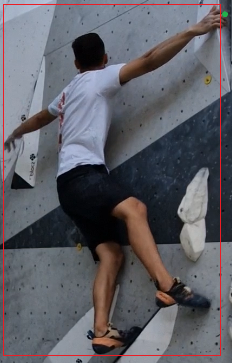
\includegraphics[width = 0.30 \textwidth]{./entities/correction_prior.png}
            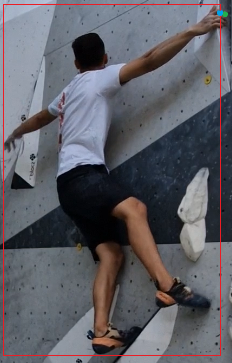
\includegraphics[width = 0.30 \textwidth]{./entities/correction_post.png}
        \end{figure}
    }
\end{frame}

\begin{frame}
    \frametitle{Conclusion}
    Succesfully developed and tested models that incorporate temporal information in 2D human pose estimation for bouldering.
    \begin{itemize}
        \item Pretraining and finetuning
        \item Multiple experiments to find the optimal setting of the models
        \item The optimal model depends on ones needs
    \end{itemize}
\end{frame}

\begin{frame}
    \frametitle{Extras: Mistakes Were Made!}
    Pretraining
    \begin{itemize}
        \item Very few overlapping samples in train/test subset
    \end{itemize}
\end{frame}

\begin{frame}
    \frametitle{Extras: Mistakes Were Made!}
    Misimplemented evaluation-function
    \begin{enumerate}
        \item<2-> Decreased accuracies
        \item<3-> Models do not improve the rough estimates
        \item<4-> bi-ConvLSTM: Model C is now always better than Model S
        \item<5-> 3DConv is generally the best performing model
    \end{enumerate}
    \begin{table}[htbp]
        \scalebox{0.7}{
            \begin{tabular}{c||ccc|ccc|ccc}
                \hline
                Accuracy metric & \multicolumn{3}{c}{PCK@0.05} & \multicolumn{3}{c}{PCK@0.1} & \multicolumn{3}{c}{PCK@0.2} \\
                \hline
                Experiment & 1 & 2 & 3 & 1 & 2 & 3 & 1 & 2 & 3 \\
                \hline
                \hline
                Identity function & 19.4 & 19.4 & 19.4 & 66.1 & 66.1 & 66.1 & 85.2 & 85.2 & 85.2 \\
                3DConv & 33.3 & 33.4 & 32.8 & 72.5 & 72.4 & 73.1 & 85.8 & 85.8 & 86.0 \\
                DeciWatch & 32.8 & 33.8 & 30.9 & 68.0 & 68.1 & 62.7 & 85.1 & 84.9 & 82.8 \\
                bi-ConvLSTM - Model S & 31.7 & 30.1 & 31.6 & 71.5 & 68.3 & 71.3 & 86.3 & 82.5 & 86.2 \\
                bi-ConvLSTM - Model C & 32.0 & 32.2 & 31.8 & 72.2 & 72.2 & 71.4 & 86.6 & 86.5 & 86.5 \\
                \hline
            \end{tabular}
        }
    \end{table}
    
    \begin{table}[htbp]
        \scalebox{0.7}{
            \begin{tabular}{c||ccc|ccc|ccc}
                \hline
                Accuracy metric & \multicolumn{3}{c}{PCK@0.05} & \multicolumn{3}{c}{PCK@0.1} & \multicolumn{3}{c}{PCK@0.2} \\
                \hline
                Experiment & 1 & 2 & 3 & 1 & 2 & 3 & 1 & 2 & 3 \\
                \hline
                \hline
                Identity function & 19.4 & 19.4 & 19.4 & 66.1 & 66.1 & 66.1 & 85.2 & 85.2 & 85.2 \\
                3DConv & 33.1 & 33.3 & 32.7 & 72.1 & 72.3 & 72.6 & 85.6 & 85.7 & 85.6 \\
                DeciWatch & 21.3 & 26.4 & 19.4 & 51.1 & 58.7 & 48.1 & 77.1 & 81.0 & 77.0 \\
                bi-ConvLSTM - Model S & 30.9 & 31.6 & 30.6 & 71.2 & 71.6 & 70.7 & 86.0 & 86.1 & 86.2 \\
                bi-ConvLSTM - Model C & 31.5 & 32.2 & 30.8 & 71.8 & 72.0 & 71.9 & 86.4 & 86.4 & 86.5 \\
                \hline
            \end{tabular}
        }
    \end{table}
\end{frame}

\begin{frame}
    \frametitle{Thanks to}
    \begin{itemize}
        \item My supervisor Kim Steenstrup Pedersen
        \item The team at ClimbAlong at NorthTech ApS
        \item My parents and my sister
    \end{itemize}
\end{frame}

\begin{frame}
    \frametitle{}
    Appendix
\end{frame}

\begin{frame}
    \frametitle{Pretraining evolution}
    \begin{figure}[htbp]
        \centering
         \begin{subfigure}[b]{\textwidth}
             \centering
             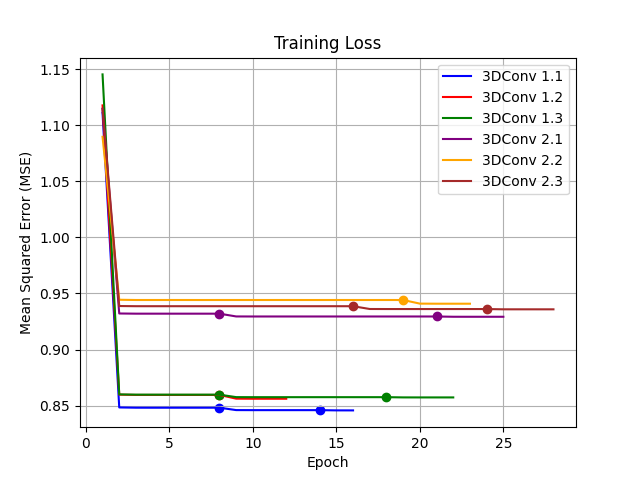
\includegraphics[width=0.32\textwidth]{../report/entities/pretrained/baseline/train_losses.png}
             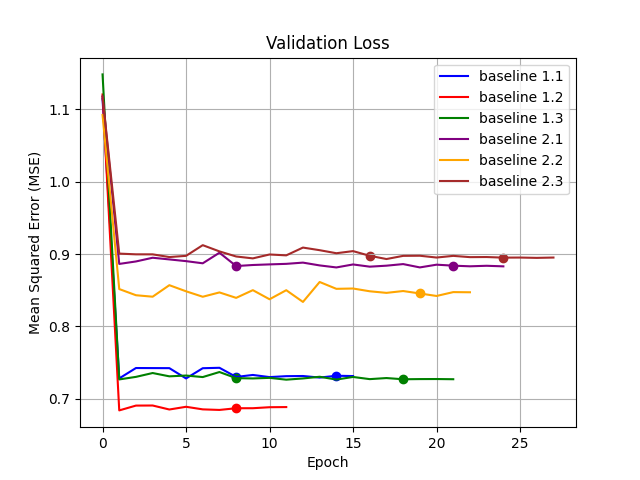
\includegraphics[width=0.32\textwidth]{../report/entities/pretrained/baseline/val_losses.png}
             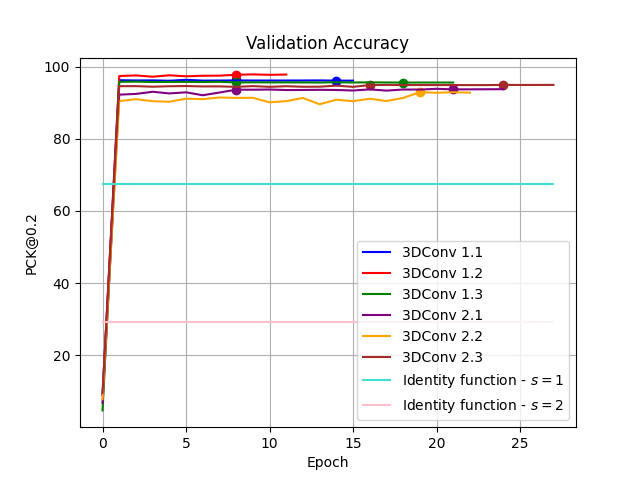
\includegraphics[width=0.32\textwidth]{../report/entities/pretrained/baseline/val_accs.png}
             \caption{Pretraining results of 3DConv.}
         \end{subfigure}
        \hfill
    
        \begin{subfigure}[b]{\textwidth}
            \centering
            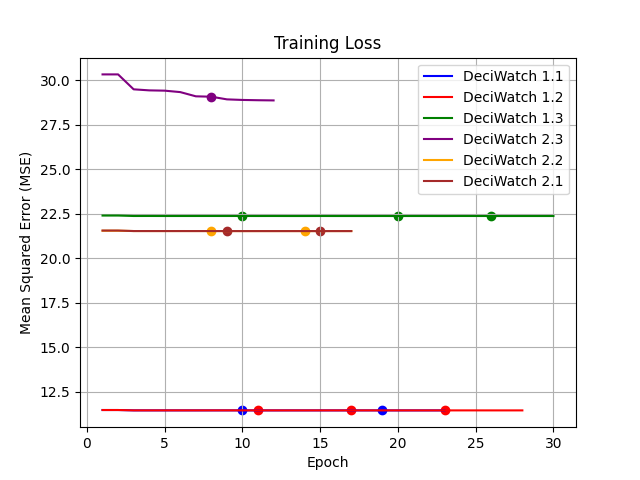
\includegraphics[width=0.32\textwidth]{../report/entities/pretrained/deciwatch/train_losses.png}
            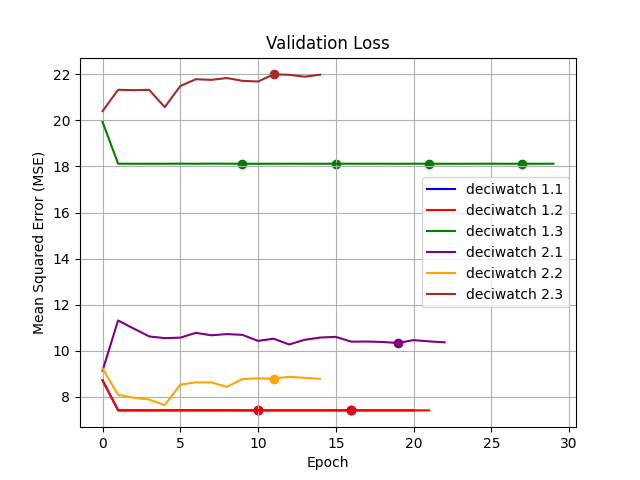
\includegraphics[width=0.32\textwidth]{../report/entities/pretrained/deciwatch/val_losses.png}
            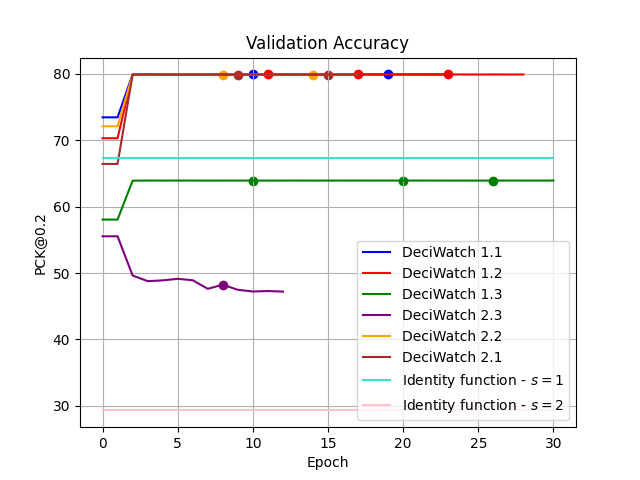
\includegraphics[width=0.32\textwidth]{../report/entities/pretrained/deciwatch/val_accs.png}
            \caption{Pretraining results of DeciWatch.}
        \end{subfigure}
       \hfill
    \end{figure}
\end{frame}

\begin{frame}
    \frametitle{Pretraining evolution}
    \begin{figure}[htbp]
        \centering
        \begin{subfigure}[b]{\textwidth}
            \centering
            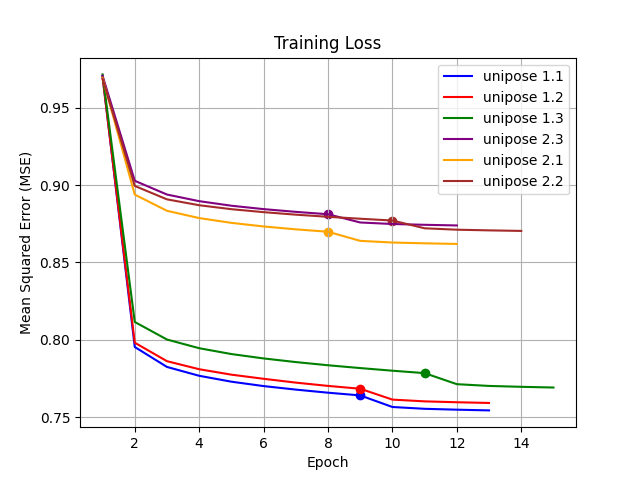
\includegraphics[width=0.32\textwidth]{../report/entities/pretrained/unipose/train_losses.png}
            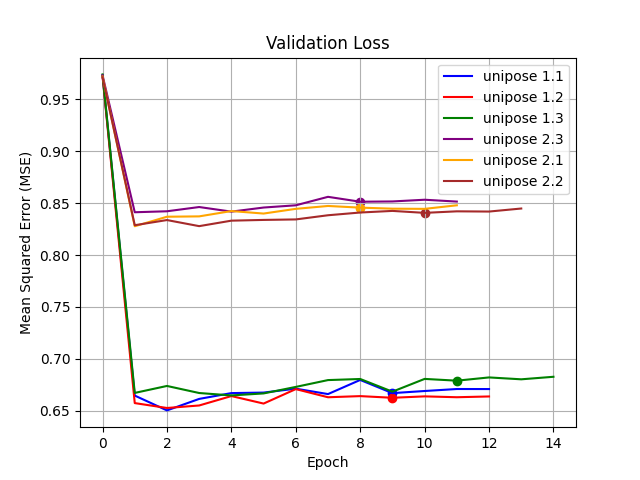
\includegraphics[width=0.32\textwidth]{../report/entities/pretrained/unipose/val_losses.png}
            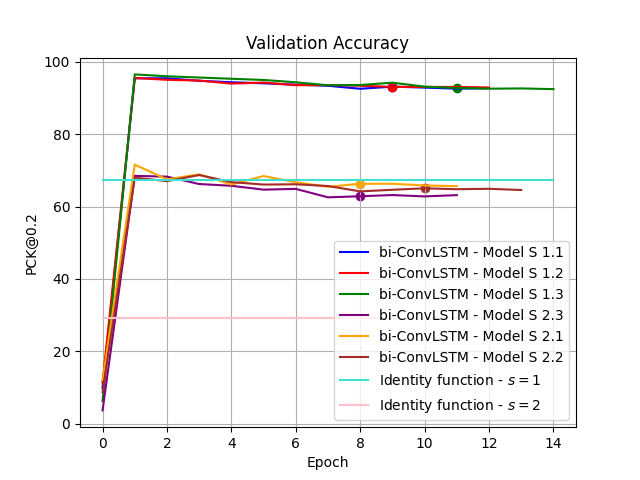
\includegraphics[width=0.32\textwidth]{../report/entities/pretrained/unipose/val_accs.png}
            \caption{Pretraining results of the bi-ConvLSTM Model S.}
        \end{subfigure}
        \hfill
        
        \begin{subfigure}[b]{\textwidth}
            \centering
            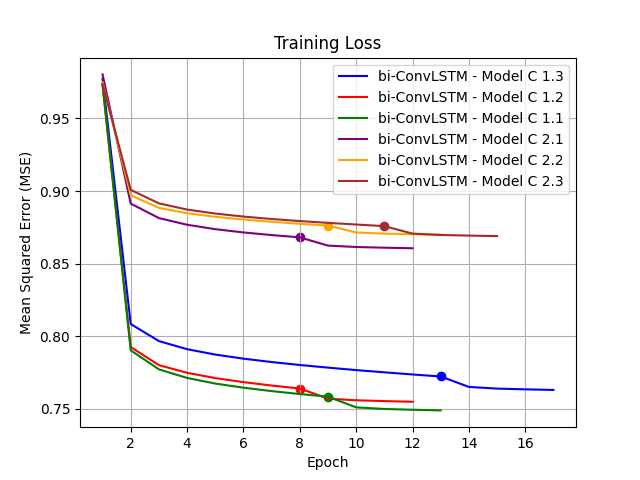
\includegraphics[width=0.32\textwidth]{../report/entities/pretrained/unipose2/train_losses.png}
            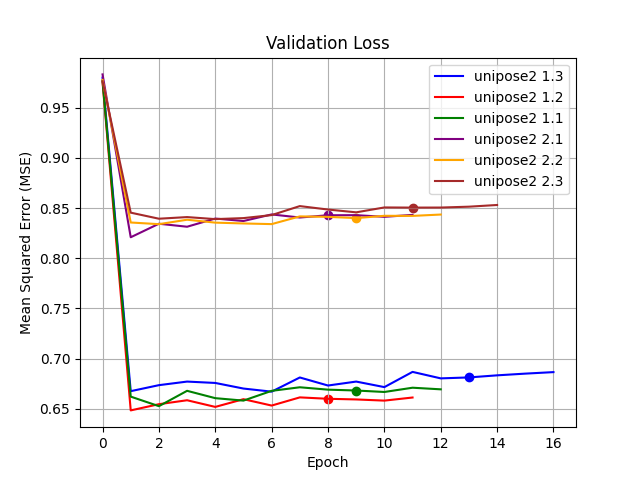
\includegraphics[width=0.32\textwidth]{../report/entities/pretrained/unipose2/val_losses.png}
            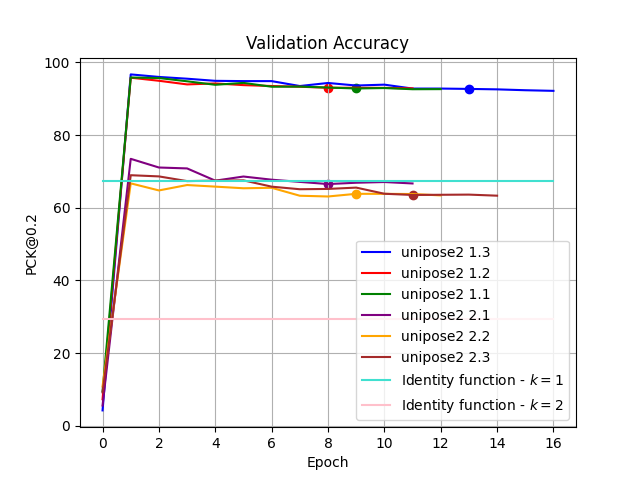
\includegraphics[width=0.32\textwidth]{../report/entities/pretrained/unipose2/val_accs.png}
            \caption{Pretraining results of the bi-ConvLSTM Model C.}
        \end{subfigure}
        \hfill
    \end{figure}
\end{frame}

\begin{frame}
    \frametitle{Pretraining test results}
    \begin{table}[htbp]
        \scalebox{0.7}{
            \begin{tabular}{c||ccc|ccc|ccc}
                \hline
                Accuracy metric & \multicolumn{3}{c}{PCK@0.05} & \multicolumn{3}{c}{PCK@0.1} & \multicolumn{3}{c}{PCK@0.2} \\
                \hline
                Mean threshold distance (px)* & \multicolumn{3}{c}{1.11} & \multicolumn{3}{c}{2.23} & \multicolumn{3}{c}{4.46} \\
                \hline
                Experiment & 1 & 2 & 3 & 1 & 2 & 3 & 1 & 2 & 3 \\
                \hline
                \hline
                Identity function & 6.95 & 6.95 & 6.95 & 25.7 & 25.7 & 25.7 & 67.4 & 67.4 & 67.4 \\
                3DConv & 1.84 & 20.5 & 0.67 & 30.6 & 58.5 & 23.8 & \textbf{96.6} & \textbf{98.0} & 96.3 \\
                DeciWatch & \textbf{51.4} & \textbf{51.4} & \textbf{44.5} & 64.6 & 64.6 & 51.5 & 80.2 & 80.2 & 64.2 \\
                bi-ConvLSTM Model S & 27.8 & 31.1 & 33.8 & 68.4 & 71.0 & \textbf{72.5} & 95.7 & 95.8 & 96.7\\
                bi-ConvLSTM Model C & 29.5 & 31.7 & 31.8 & \textbf{69.5} & \textbf{71.3} & 71.8 & 96.1 & 96.1 & \textbf{96.9} \\
                \hline
            \end{tabular}
        }
    \end{table}
    
    \begin{table}[htbp]
        \scalebox{0.7}{
            \begin{tabular}{c||ccc|ccc|ccc}
                \hline
                Accuracy metric & \multicolumn{3}{c}{PCK@0.05} & \multicolumn{3}{c}{PCK@0.1} & \multicolumn{3}{c}{PCK@0.2} \\
                \hline
                Mean threshold distance (px)* & \multicolumn{3}{c}{1.11} & \multicolumn{3}{c}{2.23} & \multicolumn{3}{c}{4.46} \\
                \hline
                Experiment & ½1 & 2 & 3 & 1 & 2 & 3 & 1 & 2 & 3 \\
                \hline
                \hline
                Identity function & 1.84 & 1.84 & 1.84 & 7.75 & 7.75 & 7.75 & 29.3 & 29.3 & 29.3 \\
                3DConv & 0.80 & 2.40 & 0.11 & 21.6 & 27.6 & 16.8 & \textbf{94.2} & \textbf{91.8} & \textbf{95.5} \\
                DeciWatch & \textbf{51.2} & \textbf{51.2} & \textbf{10.3} & \textbf{64.4} & \textbf{64.4} & 24.4 & 80.2 & 80.2 & 50.3 \\
                bi-ConvLSTM Model S & 10.5 & 11.6 & 10.1 & 31.1 & 33.4 & 29.5 & 68.5 & 67.8 & 69.6 \\
                bi-ConvLSTM Model C & 12.5 & 12.0 & 9.63 & 36.4 & 32.5 & \textbf{29.8} & 74.6 & 65.5 & 70.0 \\
                \hline
            \end{tabular}
        }
    \end{table}
\end{frame}

\begin{frame}
    \frametitle{Pretraining keypoint test results}
    \begin{table}[htbp]
        \scalebox{0.7}{
            \begin{adjustbox}{center}
                \begin{tabular}{c||ccc|ccc|ccc|ccc|c}
                    \hline
                    & \multicolumn{3}{c}{3DConv} & \multicolumn{3}{c}{DeciWatch} & \multicolumn{3}{c}{\begin{tabular}[c]{@{}c@{}}bi-ConvLSTM\\Model S\end{tabular}} & \multicolumn{3}{c}{\begin{tabular}[c]{@{}c@{}}bi-ConvLSTM\\Model C\end{tabular}} & Total \\ 
                    \hline
                    Experiment & 1 & 2 & 3 & 1 & 2 & 3 & 1 & 2 & 3 & 1 & 2 & 3 & \\
                    \hline
                    \hline
                    Nose & 30.4 & 44.3 & 26.5 & 68.9 & 68.0 & 54.1 & 80.6 & 67.7 & 81.4 & 74.9 & 73.3 & 70.1 & 61.7 \\
                    Ear & 29.4 & 43.8 & 24.9 & 69.6 & 69.6 & 55.2 & 76.5 & 73.2 & 76.2 & 74.9 & 75.2 & 71.5 & 61.7 \\
                    Shoulder & 34.0 & 71.3 & 29.4 & 68.1 & 68.1 & 53.5 & 65.2 & 72.0 & 71.4 & 70.9 & 77.0 & 69.4 & 62.5 \\
                    Elbow & 31.1 & 68.3 & 24.0 & 62.7 & 62.7 & 49.4 & 71.9 & 79.0 & 68.0 & 67.6 & 71.9 & 83.6 & 61.7 \\
                    Wrist & 26.5 & 45.3 & 19.8 & 59.8 & 59.8 & 48.3 & 70.5 & 70.4 & 66.8 & 68.6 & 70.7 & 74.6 & 56.8 \\
                    Hip & 34.3 & 84.3 & 24.4 & 63.6 & 63.6 & 50.1 & 65.2 & 65.6 & 57.4 & 67.1 & 62.1 & 56.3 & 57.8 \\
                    Knee & 33.7 & 65.2 & 25.1 & 59.5 & 59.5 & 48.0 & 73.9 & 69.2 & 66.8 & 61.9 & 69.0 & 73.2 & 58.8 \\
                    Ankle & 25.4 & 37.2 & 17.6 & 58.9 & 58.9 & 48.3 & 80.1 & 69.4 & 66.1 & 73.1 & 72.2 & 75.2 & 56.9 \\
                    \hline
                    Total & 30.6 & 58.5 & 23.8 & 64.6 & 64.6 & 51.5 & 68.4 & 71.0 & 72.5 & 69.5 & 71.3 & 71.8 & \\
                    \hline
                \end{tabular}
            \end{adjustbox}
        }
    \end{table}
    
    \begin{table}[htbp]
        \scalebox{0.7}{
            \begin{adjustbox}{center}
                \begin{tabular}{c||ccc|ccc|ccc|ccc|c}
                    \hline
                    & \multicolumn{3}{c}{3DConv} & \multicolumn{3}{c}{DeciWatch} & \multicolumn{3}{c}{\begin{tabular}[c]{@{}c@{}}bi-ConvLSTM\\Model S\end{tabular}} & \multicolumn{3}{c}{\begin{tabular}[c]{@{}c@{}}bi-ConvLSTM\\Model C\end{tabular}} & Total \\ 
                    \hline
                    Experiment & 1 & 2 & 3 & 1 & 2 & 3 & 1 & 2 & 3 & 1 & 2 & 1.3 & \\
                    \hline
                    \hline
                    Nose & 20.5 & 20.5 & 17.3 & 67.9 & 22.2 & 41.8 & 75.8 & 36.2 & 29.1 & 32.8 & 35.2 & 25.5 & 35.4 \\
                    Ear & 22.5 & 29.7 & 18.8 & 69.1 & 18.6 & 47.9 & 80.3 & 46.9 & 42.7 & 47.9 & 49.4 & 42.4 & 43.0 \\
                    Shoulder & 22.4 & 30.5 & 17.0 & 68.1 & 13.3 & 32.2 & 74.7 & 26.3 & 23.3 & 32.8 & 31.5 & 21.0 & 32.8 \\
                    Elbow & 22.5 & 32.0 & 16.5 & 62.7 & 14.1 & 19.3 & 58.2 & 33.9 & 21.1 & 27.2 & 31.1 & 27.1 & 30.5 \\
                    Wrist & 21.5 & 26.9 & 17.1 & 59.7 & 34.2 & 35.5 & 69.4 & 37.1 & 32.3 & 39.8 & 33.1 & 33.5 & 36.7 \\
                    Hip & 22.4 & 27.9 & 16.3 & 63.5 & 16.8 & 19.9 & 64.7 & 26.5 & 32.1 & 35.2 & 22.2 & 30.3 & 31.5 \\
                    Knee & 19.9 & 25.5 & 15.4 & 59.5 & 24.2 & 23.4 & 60.1 & 28.2 & 16.1 & 26.0 & 21.0 & 13.2 & 27.7 \\
                    Ankle & 21.0 & 24.5 & 16.2 & 58.8 & 47.5 & 35.6 & 69.4 & 34.1 & 40.0 & 48.6 & 39.4 & 43.7 & 39.9 \\
                    \hline
                    Total & 21.6 & 27.6 & 16.8 & 64.4 & 64.4 & 24.4 & 31.1 & 33.4 & 29.5 & 36.4 & 32.5 & 29.8 & \\
                    \hline
                \end{tabular}
            \end{adjustbox}
        }
    \end{table}
\end{frame}

\begin{frame}
    \frametitle{Finetuning evolution}
    \begin{figure}[htbp]
        \centering
         \begin{subfigure}[b]{\textwidth}
             \centering
             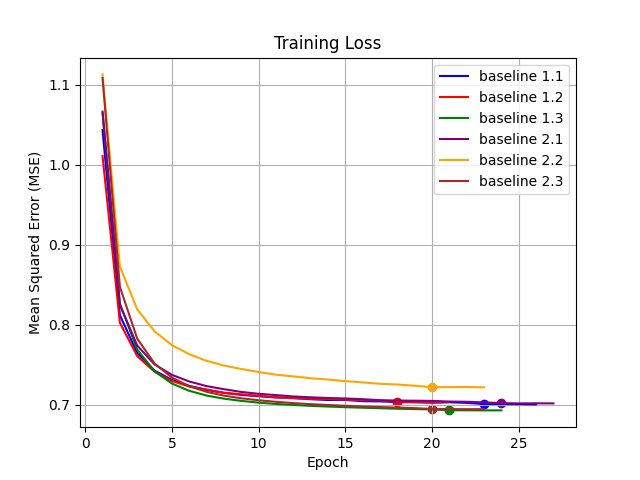
\includegraphics[width=0.32\textwidth]{../report/entities/finetuned/baseline/train_losses.png}
             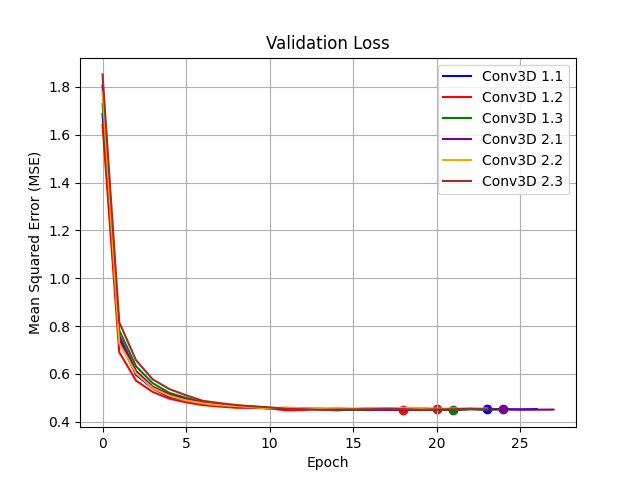
\includegraphics[width=0.32\textwidth]{../report/entities/finetuned/baseline/val_losses.png}
             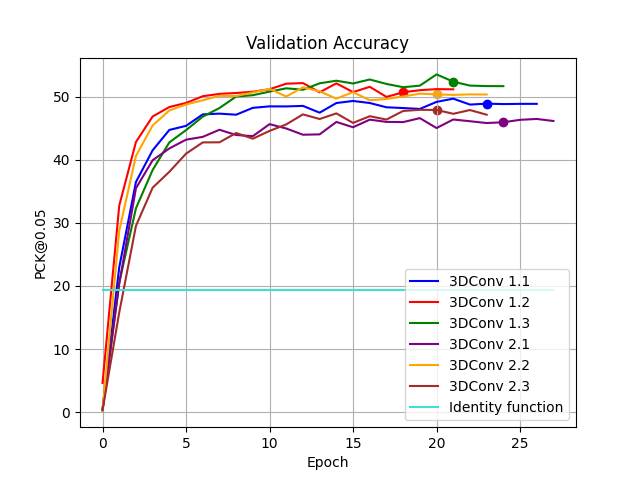
\includegraphics[width=0.32\textwidth]{../report/entities/finetuned/baseline/val_accs.png}
             \caption{Finetuning results of 3DConv.}
         \end{subfigure}
        \hfill
    
        \begin{subfigure}[b]{\textwidth}
            \centering
            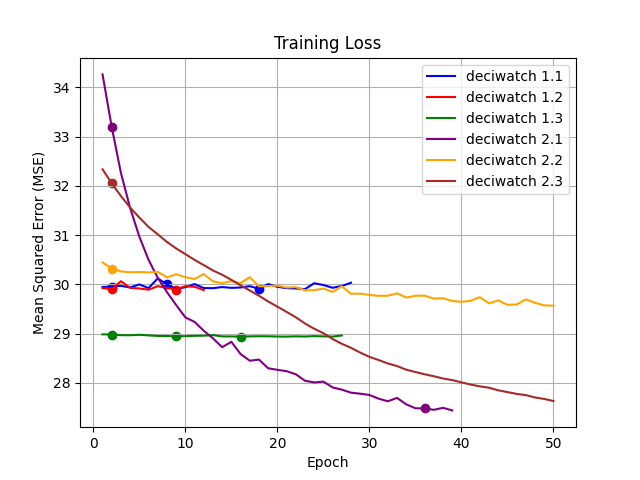
\includegraphics[width=0.32\textwidth]{../report/entities/finetuned/deciwatch/train_losses.png}
            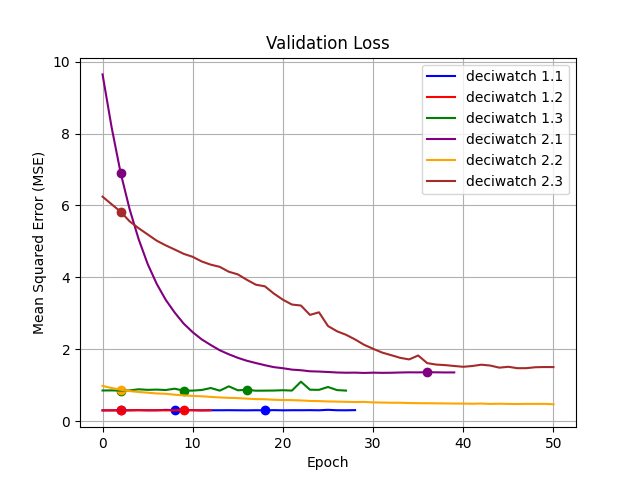
\includegraphics[width=0.32\textwidth]{../report/entities/finetuned/deciwatch/val_losses.png}
            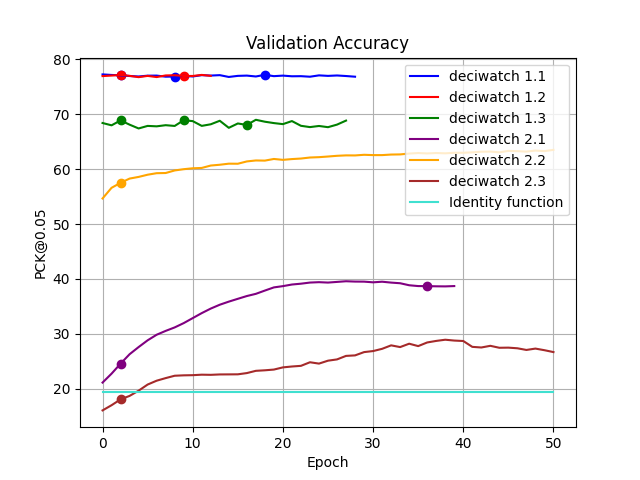
\includegraphics[width=0.32\textwidth]{../report/entities/finetuned/deciwatch/val_accs.png}
            \caption{Finetuning results of DeciWatch.}
        \end{subfigure}
       \hfill
    \end{figure}
\end{frame}

\begin{frame}
    \frametitle{Finetuning evolution}
    \begin{figure}[htbp]
        \centering    
        \begin{subfigure}[b]{\textwidth}
            \centering
            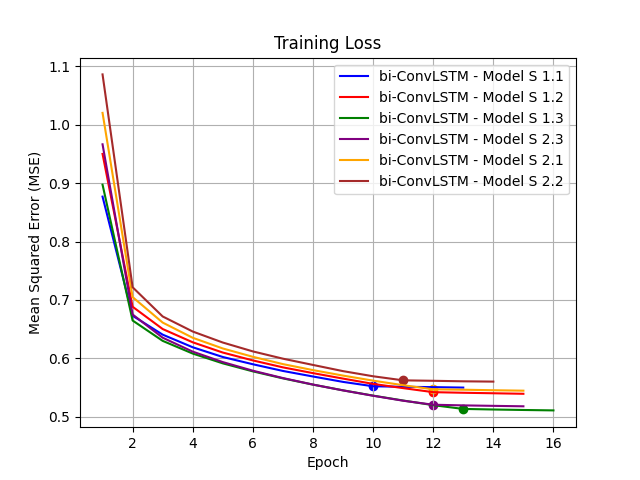
\includegraphics[width=0.32\textwidth]{../report/entities/finetuned/unipose/train_losses.png}
            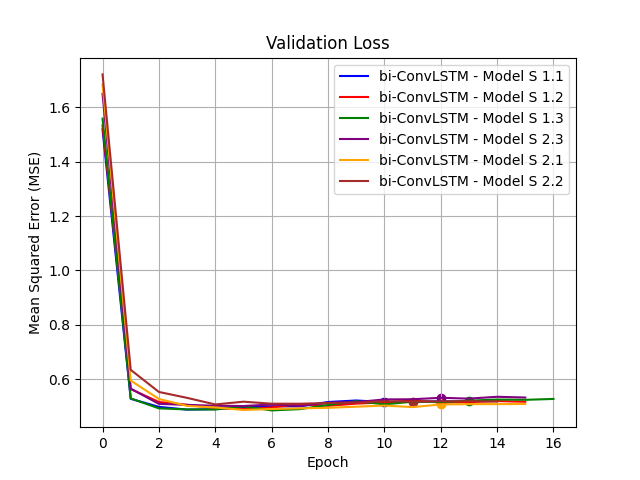
\includegraphics[width=0.32\textwidth]{../report/entities/finetuned/unipose/val_losses.png}
            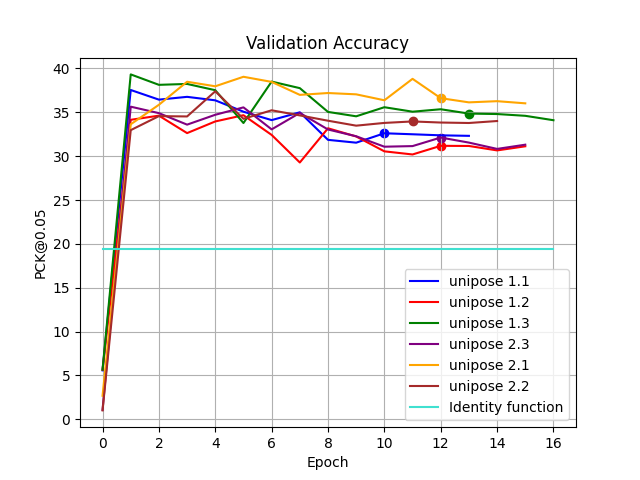
\includegraphics[width=0.32\textwidth]{../report/entities/finetuned/unipose/val_accs.png}
            \caption{Finetuning results of bi-Conv LSTM Model S.}
        \end{subfigure}
        \hfill
    
        \begin{subfigure}[b]{\textwidth}
            \centering
            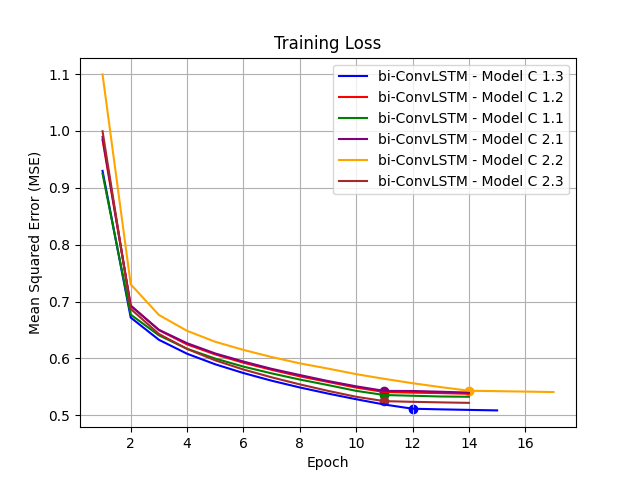
\includegraphics[width=0.32\textwidth]{../report/entities/finetuned/unipose2/train_losses.png}
            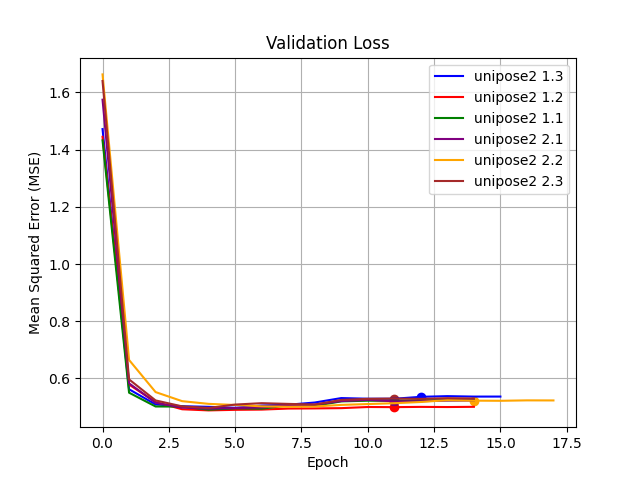
\includegraphics[width=0.32\textwidth]{../report/entities/finetuned/unipose2/val_losses.png}
            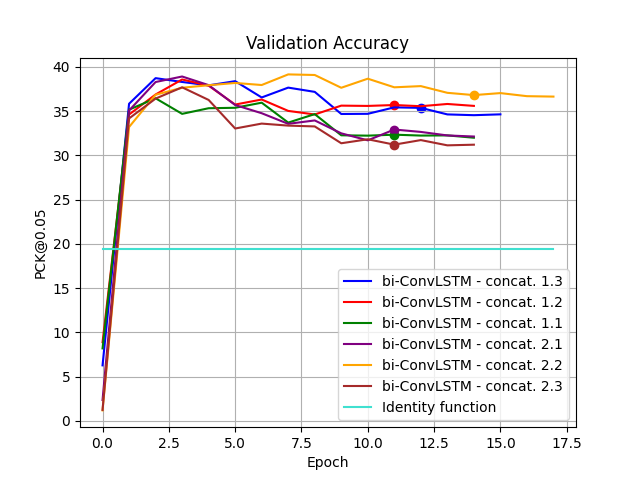
\includegraphics[width=0.32\textwidth]{../report/entities/finetuned/unipose2/val_accs.png}
            \caption{Finetuning results of bi-Conv LSTM Model C.}
        \end{subfigure}
        \hfill
    \end{figure}
\end{frame}

\begin{frame}
    \frametitle{Finetuning evolution with regularization}
    \begin{figure}
        \centering
        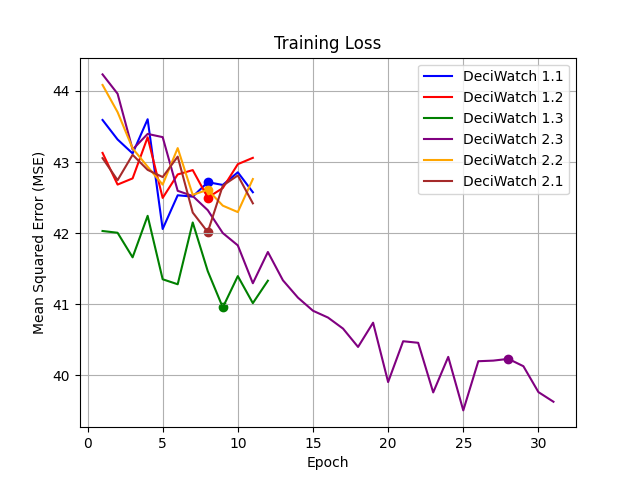
\includegraphics[width=0.32\textwidth]{../report/entities/finetuned/adapted/train_losses.png}
        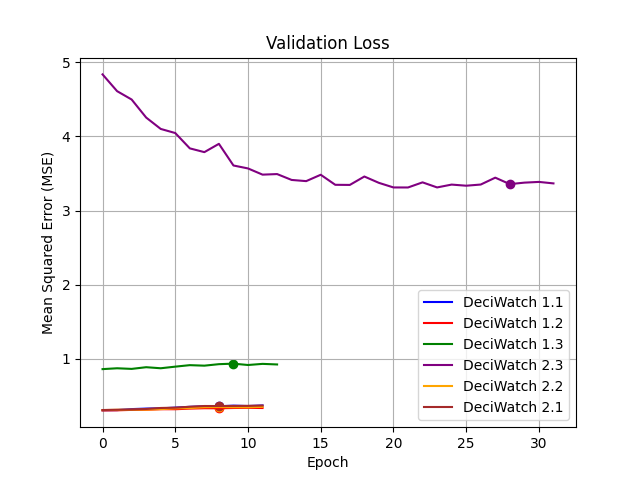
\includegraphics[width=0.32\textwidth]{../report/entities/finetuned/adapted/val_losses.png}
        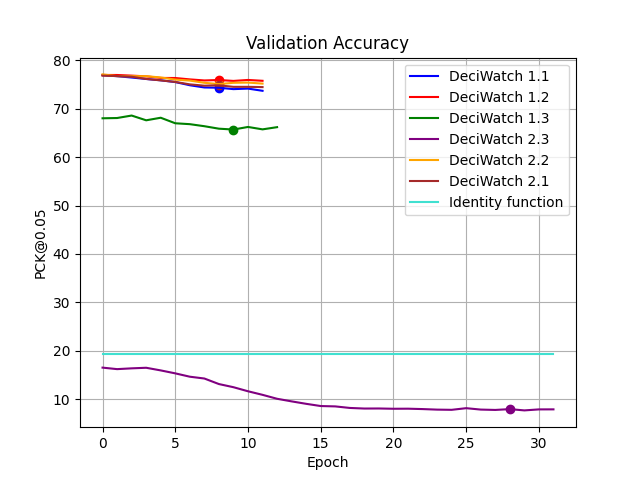
\includegraphics[width=0.32\textwidth]{../report/entities/finetuned/adapted/val_accs.png}
    \end{figure}
\end{frame}

\begin{frame}
    \frametitle{Finetuning test results}
    \begin{table}[htbp]
        \scalebox{0.7}{
            \begin{tabular}{c||ccc|ccc|ccc}
                \hline
                Accuracy metric & \multicolumn{3}{c}{PCK@0.05} & \multicolumn{3}{c}{PCK@0.1} & \multicolumn{3}{c}{PCK@0.2} \\
                \hline
                Mean threshold distance (px)* & \multicolumn{3}{c}{0.80} & \multicolumn{3}{c}{1.60} & \multicolumn{3}{c}{3.21} \\
                \hline
                Experiment & 1 & 2 & 3 & 1 & 2 & 3 & 1 & 2 & 3 \\
                \hline
                \hline
                Identity function & 19.4 & 19.4 & 19.4 & 66.1 & 66.1 & 66.1 & 85.2 & 85.2 & 85.2 \\
                3DConv & 49.7 & 52.3 & 53.1 & \textbf{95.7} & \textbf{95.7} & \textbf{95.8} & 99.2 & 99.3 & 99.3 \\
                DeciWatch & \textbf{76.6} & \textbf{76.7} & \textbf{68.1} & 94.4 & 94.3 & 87.3 & 99.2 & 99.2 & 96.1 \\
                bi-ConvLSTM - Model S & 37.8 & 34.9 & 39.0 & 91.8 & 92.1 & 92.2 & 99.4 & \textbf{99.7} & 99.2 \\
                bi-ConvLSTM - Model C & 35.9 & 39.0 & 38.5 & 93.1 & 93.6 & 92.6 & \textbf{99.8} & \textbf{99.7} & \textbf{99.7} \\
                \hline
            \end{tabular}
        }
    \end{table}
    
    \begin{table}[htbp]
        \scalebox{0.7}{
            \begin{tabular}{c||ccc|ccc|ccc}
                \hline
                Accuracy metric & \multicolumn{3}{c}{PCK@0.05} & \multicolumn{3}{c}{PCK@0.1} & \multicolumn{3}{c}{PCK@0.2} \\
                \hline
                Mean threshold distance (px)* & \multicolumn{3}{c}{0.80} & \multicolumn{3}{c}{1.60} & \multicolumn{3}{c}{3.21} \\
                \hline
                Experiment & 1 & 2 & 3 & 1 & 2 & 3 & 1 & 2 & 3 \\
                \hline
                \hline
                Identity function & 19.4 & 19.4 & 19.4 & 66.1 & 66.1 & 66.1 & 85.2 & 85.2 & 85.2 \\
                3DConv & 46.5 & 51.6 & \textbf{47.3} & \textbf{95.5} & \textbf{95.5} & \textbf{95.8} & 99.2 & 99.3 & 99.2 \\
                DeciWatch & \textbf{76.0} & \textbf{75.9} & 36.8 & 94.2 & 94.2 & 74.9 & 99.2 & 99.2 & 92.8 \\
                bi-ConvLSTM - Model S & 38.8 & 37.4 & 35.9 & 92.7 & 92.1 & 91.2 & 99.4 & \textbf{99.5} & 99.3 \\
                bi-ConvLSTM - Model C & 39.2 & 39.5 & 37.1 & 92.5 & 92.9 & 92.6 & \textbf{99.6} & 99.3 & \textbf{99.6} \\
                \hline
            \end{tabular}
        }
    \end{table}
\end{frame}

\begin{frame}
    \frametitle{Finetuning additional test results}
    \begin{table}[htbp]
        \scalebox{0.7}{
            \begin{tabular}{c||ccc|ccc|ccc}
                \hline
                Accuracy metric & \multicolumn{3}{c}{PCK@0.05} & \multicolumn{3}{c}{PCK@0.1} & \multicolumn{3}{c}{PCK@0.2} \\
                \hline
                Mean threshold distance* & \multicolumn{3}{c}{0.87} & \multicolumn{3}{c}{1.77} & \multicolumn{3}{c}{3.55} \\
                \hline
                Experiment & 1 & 2 & 3 & 1 & 2 & 3 & 1 & 2 & 3 \\
                \hline
                \hline
                Identity function & 21.2 & 21.2 & 21.2 & 65.5 & 65.5 & 65.5 & 84.7 & 84.7 & 84.7 \\
                3DConv & 58.4 & 61.4 & 61.7 & \textbf{98.7} & \textbf{98.9} & \textbf{99.0} & \textbf{99.6} & \textbf{99.8} & \textbf{99.7} \\
                DeciWatch & \textbf{82.6} & \textbf{82.4} & \textbf{74.6} & 96.2 & 96.1 & 92.3 & 99.1 & 99.1 & 97.4 \\
                bi-ConvLSTM - Model S & 45.7 & 45.0 & 47.6 & 97.3 & 96.9 & 97.0 & \textbf{99.6} & 99.6 & 99.1 \\
                bi-ConvLSTM - Model C & 44.5 & 46.1 & 48.5 & 97.4 & 97.9 & 97.9 & 99.6 & 99.5 & 99.6 \\
                \hline
            \end{tabular}
        }
    \end{table}
    
    \begin{table}[htbp]
        \scalebox{0.7}{
            \begin{tabular}{c||ccc|ccc|ccc}
                \hline
                Accuracy metric & \multicolumn{3}{c}{PCK@0.05} & \multicolumn{3}{c}{PCK@0.1} & \multicolumn{3}{c}{PCK@0.2} \\
                \hline
                Mean threshold distance* & \multicolumn{3}{c}{0.87} & \multicolumn{3}{c}{1.77} & \multicolumn{3}{c}{3.55} \\
                \hline
                Experiment & 1 & 2 & 3 & 1 & 2 & 3 & 1 & 2 & 3 \\
                \hline
                \hline
                Identity function & 21.2 & 21.2 & 21.2 & 65.5 & 65.5 & 65.5 & 84.7 & 84.7 & 84.7 \\
                3DConv & 56.2 & 60.0 & \textbf{56.6} & \textbf{98.9} & \textbf{98.8} & \textbf{98.8} & \textbf{99.7} & \textbf{99.7} & \textbf{99.7} \\
                DeciWatch & \textbf{81.6} & \textbf{81.8} & 37.5 & 96.0 & 96.0 & 73.3 & 99.1 & 99.1 & 90.7 \\
                bi-ConvLSTM - Model S & 44.8 & 46.2 & 45.0 & 96.9 & 95.9 & 97.1 & 99.5 & 99.6 & 99.5 \\
                bi-ConvLSTM - Model C & 45.9 & 47.9 & 46.7 & 96.7 & 97.1 & 98.1 & 99.6 & 99.4 & 99.6 \\
                \hline
            \end{tabular}
        }
    \end{table}
\end{frame}

\begin{frame}
    \frametitle{Finetuning keypoint testing results}
    \begin{table}[htbp]
        \scalebox{0.7}{
            \begin{adjustbox}{center}
                \begin{tabular}{c||ccc|ccc|ccc|ccc|c}
                    \hline
                    & \multicolumn{3}{c}{3DConv} & \multicolumn{3}{c}{DeciWatch} & \multicolumn{3}{c}{\begin{tabular}[c]{@{}c@{}}bi-ConvLSTM\\ Model S\end{tabular}} & \multicolumn{3}{c}{\begin{tabular}[c]{@{}c@{}}bi-ConvLSTM\\ Model C\end{tabular}} & Total \\ 
                    \hline
                    Experiment & 1 & 2 & 3 & 1 & 2 & 3 & 1 & 2 & 3 & 1 & 2 & 3 & \\
                    \hline
                    \hline
                    Nose & 95.5 & 97.6 & 95.7 & 94.9 & 94.9 & 88.5 & 93.5 & 89.7 & 95.4 & 93.4 & 88.8 & 90.9 & 93.2 \\
                    Ear & 96.5 & 96.7 & 96.8 & 95.5 & 95.5 & 88.6 & 94.3 & 91.9 & 94.2 & 96.3 & 95.6 & 96.1 & 94.8 \\
                    Shoulder & 95.6 & 97.4 & 97.1 & 95.4 & 95.4 & 88.4 & 91.2 & 90.6 & 87.2 & 91.9 & 95.1 & 92.9 & 93.2 \\
                    Elbow & 97.6 & 97.2 & 97.5 & 94.5 & 94.6 & 86.5 & 93.2 & 93.7 & 94.9 & 95.1 & 96.7 & 95.2 & 94.7 \\
                    Wrist & 96.4 & 96.4 & 96.3 & 93.9 & 93.9 & 85.8 & 94.2 & 92.7 & 94.1 & 94.5 & 93.2 & 94.3 & 93.8 \\
                    Pinky & 86.6 & 85.4 & 85.4 & 92.5 & 92.2 & 84.0 & 84.5 & 86.5 & 86.6 & 83.4 & 88.4 & 87.0 & 86.9 \\
                    Index finger & 92.7 & 92.5 & 93.1 & 92.2 & 92.1 & 84.3 & 90.3 & 89.1 & 88.2 & 89.9 & 92.3 & 92.1 & 90.7 \\
                    Thumb & 91.6 & 91.0 & 91.4 & 92.8 & 92.7 & 84.5 & 81.0 & 89.3 & 84.9 & 89.6 & 85.5 & 86.9 & 88.4 \\
                    Hip & 99.4 & 99.0 & 99.8 & 96.4 & 96.4 & 89.9 & 92.5 & 96.5 & 98.0 & 94.6 & 97.7 & 96.1 & 96.4 \\
                    Knee & 97.7 & 98.1 & 98.4 & 95.0 & 95.0 & 88.4 & 96.1 & 92.5 & 96.5 & 96.0 & 93.9 & 93.6 & 95.1 \\
                    Ankle & 98.6 & 98.4 & 99.1 & 95.0 & 95.0 & 87.6 & 94.3 & 93.6 & 96.0 & 97.2 & 98.1 & 94.3 & 95.6 \\
                    Heel & 98.6 & 98.1 & 98.5 & 95.2 & 95.1 & 86.2 & 94.2 & 93.4 & 94.9 & 92.5 & 92.6 & 93.0 & 94.4 \\
                    Toes & 97.2 & 97.5 & 98.0 & 94.2 & 94.0 & 86.8 & 94.9 & 95.3 & 95.5 & 93.8 & 95.7 & 94.4 & 94.8 \\
                    \hline
                    Total & 95.7 & 95.7 & 95.8 & 94.4 & 94.3 & 87.3 & 91.8 & 92.1 & 92.2 & 93.1 & 93.6 & 92.6 & \\
                    \hline
                \end{tabular}
            \end{adjustbox}
        }
    \end{table}
\end{frame}

\begin{frame}
    \frametitle{Finetuning keypoint testing results}
    
    \begin{table}[htbp]
        \scalebox{0.7}{
            \begin{adjustbox}{center}
                \begin{tabular}{c||ccc|ccc|ccc|ccc|c}
                    \hline
                    & \multicolumn{3}{c}{3DConv} & \multicolumn{3}{c}{DeciWatch} & \multicolumn{3}{c}{\begin{tabular}[c]{@{}c@{}}bi-ConvLSTM\\ Model S\end{tabular}} & \multicolumn{3}{c}{\begin{tabular}[c]{@{}c@{}}bi-ConvLSTM\\ Model C\end{tabular}} & Total \\ 
                    \hline
                    Experiment & 1.1 & 1.2 & 1.3 & 1.1 & 1.2 & 1.3 & 1.1 & 1.2 & 1.3 & 1.1 & 1.2 & 1.3 & \\
                    \hline
                    \hline
                    Nose & 95.6 & 97.0 & 95.6 & 94.1 & 94.3 & 80.8 & 90.9 & 89.6 & 93.2 & 88.1 & 91.1 & 90.8 & 91.76 \\
                    Ear & 96.8 & 95.7 & 96.9 & 93.3 & 93.4 & 80.8 & 94.2 & 92.7 & 92.6 & 91.9 & 93.2 & 94.9 & 93.0 \\
                    Shoulder & 95.1 & 97.1 & 95.7 & 95.3 & 95.4 & 77.5 & 93.5 & 93.4 & 90.1 & 90.0 & 97.7 & 95.6 & 93.0 \\
                    Elbow & 97.2 & 97.1 & 97.5 & 94.4 & 94.5 & 72.0 & 96.0 & 96.7 & 90.9 & 97.1 & 97.0 & 94.7 & 93.8 \\
                    Wrist & 96.4 & 96.5 & 96.6 & 93.8 & 93.8 & 77.4 & 89.2 & 93.8 & 91.9 & 93.2 & 94.3 & 9.33 & 85.5 \\
                    Pinky & 85.0 & 85.3 & 87.0 & 92.3 & 92.4 & 66.1 & 84.5 & 82.6 & 84.0 & 87.4 & 83.6 & 89.7 & 85.0 \\
                    Index finger & 93.1 & 92.8 & 93.0 & 92.5 & 92.5 & 65.3 & 92.7 & 89.9 & 92.4 & 92.1 & 88.0 & 91.4 & 89.6 \\
                    Thumb & 91.1 & 90.8 & 91.6 & 93.0 & 92.9 & 71.4 & 85.3 & 83.5 & 81.1 & 82.6 & 84.6 & 88.9 & 86.4 \\
                    Hip & 99.3 & 98.8 & 99.6 & 96.3 & 96.4 & 78.6 & 97.1 & 96.2 & 96.8 & 97.8 & 97.4 & 84.5 & 94.9 \\
                    Knee & 97.6 & 97.8 & 97.9 & 95.1 & 95.0 & 77.9 & 94.9 & 93.3 & 91.3 & 95.9 & 98.4 & 97.5 & 94.4 \\
                    Ankle & 98.6 & 98.5 & 99.3 & 94.5 & 94.6 & 79.3 & 96.2 & 96.0 & 93.8 & 98.5 & 96.8 & 96.2 & 95.2 \\
                    Heel & 98.2 & 97.8 & 98.8 & 95.1 & 95.0 & 78.5 & 93.7 & 93.0 & 93.2 & 93.0 & 91.3 & 92.8 & 93.4 \\
                    Toes & 97.4 & 97.4 & 97.8 & 94.0 & 94.0 & 73.1 & 95.1 & 96.8 & 93.5 & 92.7 & 93.7 & 93.7 & 93.3 \\
                    \hline
                    Total & 95.5 & 95.5 & 95.8 & 94.2 & 94.2 & 74.9 & 92.7 & 92.1 & 91.2 & 92.5 & 92.9 & 92.6 & \\
                    \hline
                \end{tabular}
            \end{adjustbox}
        }
    \end{table}
\end{frame}

\begin{frame}
    \frametitle{Pretraining evolution - corrected}
    \begin{figure}[htbp]
        \centering    
        \begin{subfigure}[b]{\textwidth}
            \centering
            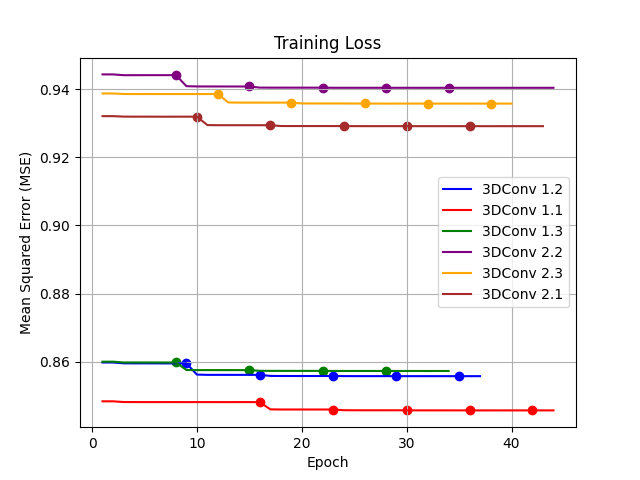
\includegraphics[width=0.32\textwidth]{./entities/pretrained_new/baseline/train_losses.png}
            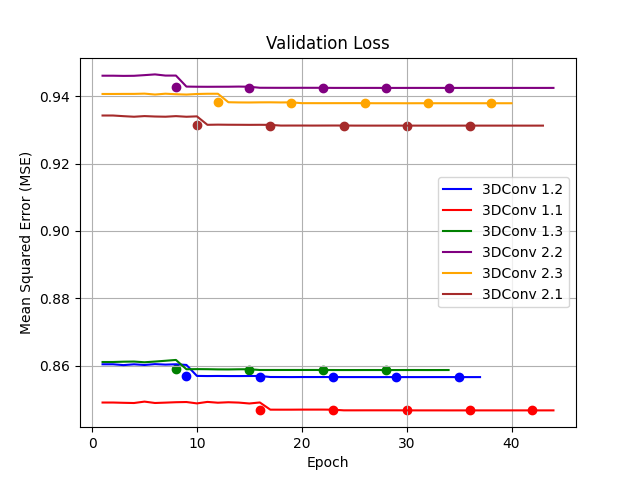
\includegraphics[width=0.32\textwidth]{./entities/pretrained_new/baseline/val_losses.png}
            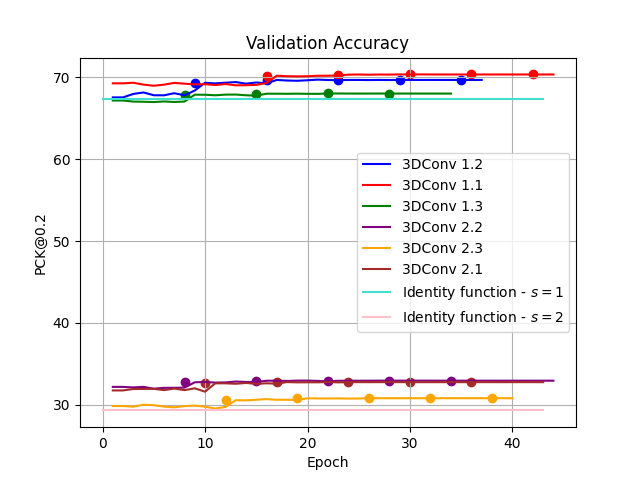
\includegraphics[width=0.32\textwidth]{./entities/pretrained_new/baseline/val_accs.png}
            \caption{Pretraining results of 3DConv}
        \end{subfigure}
        \hfill
    
        \begin{subfigure}[b]{\textwidth}
            \centering
            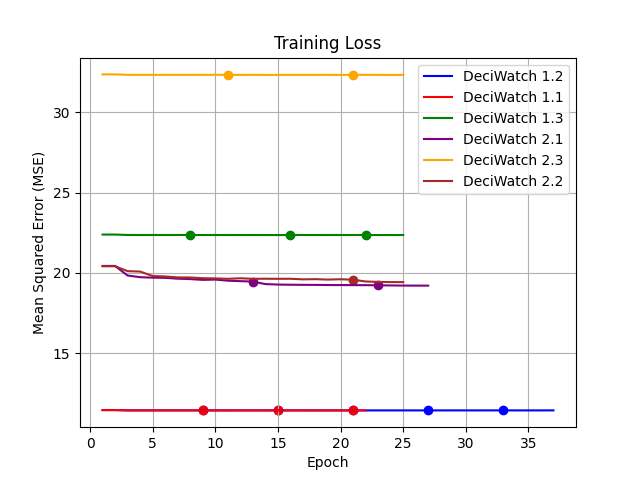
\includegraphics[width=0.32\textwidth]{./entities/pretrained_new/deciwatch/train_losses.png}
            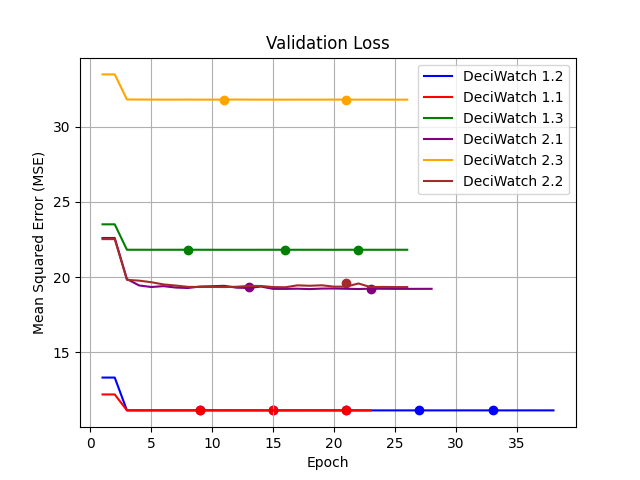
\includegraphics[width=0.32\textwidth]{./entities/pretrained_new/deciwatch/val_losses.png}
            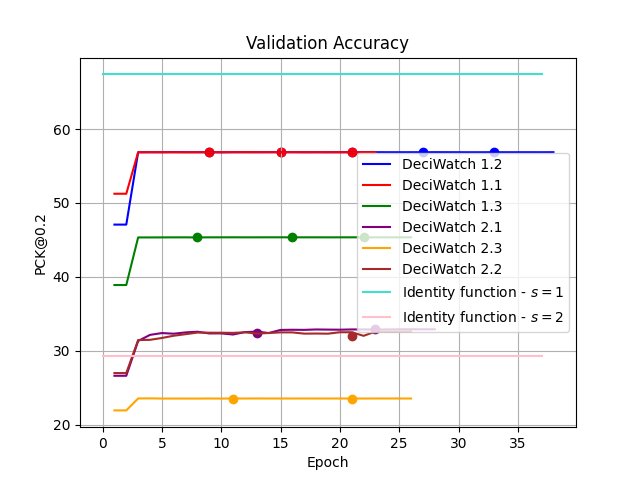
\includegraphics[width=0.32\textwidth]{./entities/pretrained_new/deciwatch/val_accs.png}
            \caption{Pretraining results of DeciWatch}
        \end{subfigure}
        \hfill
    \end{figure}
\end{frame}

\begin{frame}
    \frametitle{Pretraining evolution - corrected}
    \begin{figure}[htbp]
        \centering    
        \begin{subfigure}[b]{\textwidth}
            \centering
            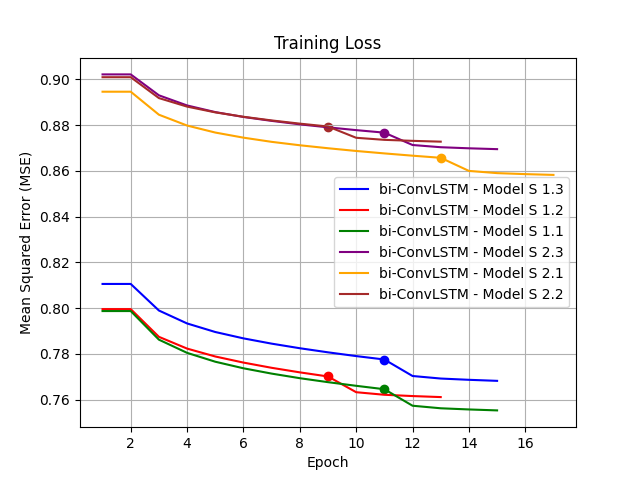
\includegraphics[width=0.32\textwidth]{./entities/pretrained_new/unipose/train_losses.png}
            \includegraphics[width=0.32\textwidth]{./entities/pretrained_new/unipose/val_losses.png}
            \includegraphics[width=0.32\textwidth]{./entities/pretrained_new/unipose/val_accs.png}
            \caption{Pretraining results of bi-Conv LSTM Model S.}
        \end{subfigure}
        \hfill
    
        \begin{subfigure}[b]{\textwidth}
            \centering
            \includegraphics[width=0.32\textwidth]{./entities/pretrained_new/unipose2/train_losses.png}
            \includegraphics[width=0.32\textwidth]{./entities/pretrained_new/unipose2/val_losses.png}
            \includegraphics[width=0.32\textwidth]{./entities/pretrained_new/unipose2/val_accs.png}
            \caption{Pretraining results of bi-Conv LSTM Model C.}
        \end{subfigure}
        \hfill
    \end{figure}
\end{frame}

\begin{frame}
    \frametitle{Finetuning evolution - corrected}
    \begin{figure}[htbp]
        \centering    
        \begin{subfigure}[b]{\textwidth}
            \centering
            \includegraphics[width=0.32\textwidth]{./entities/finetuned_new/baseline/train_losses.png}
            \includegraphics[width=0.32\textwidth]{./entities/finetuned_new/baseline/val_losses.png}
            \includegraphics[width=0.32\textwidth]{./entities/finetuned_new/baseline/val_accs.png}
            \caption{Finetuning results of 3DConv}
        \end{subfigure}
        \hfill
    
        \begin{subfigure}[b]{\textwidth}
            \centering
            \includegraphics[width=0.32\textwidth]{./entities/finetuned_new/deciwatch/train_losses.png}
            \includegraphics[width=0.32\textwidth]{./entities/finetuned_new/deciwatch/val_losses.png}
            \includegraphics[width=0.32\textwidth]{./entities/finetuned_new/deciwatch/val_accs.png}
            \caption{Finetuning results of DeciWatch}
        \end{subfigure}
        \hfill
    \end{figure}
\end{frame}

\begin{frame}
    \frametitle{Finetuning evolution - corrected}
    \begin{figure}[htbp]
        \centering    
        \begin{subfigure}[b]{\textwidth}
            \centering
            \includegraphics[width=0.32\textwidth]{./entities/finetuned_new/unipose/train_losses.png}
            \includegraphics[width=0.32\textwidth]{./entities/finetuned_new/unipose/val_losses.png}
            \includegraphics[width=0.32\textwidth]{./entities/finetuned_new/unipose/val_accs.png}
            \caption{Finetuning results of bi-Conv LSTM Model S.}
        \end{subfigure}
        \hfill
    
        \begin{subfigure}[b]{\textwidth}
            \centering
            \includegraphics[width=0.32\textwidth]{./entities/finetuned_new/unipose2/train_losses.png}
            \includegraphics[width=0.32\textwidth]{./entities/finetuned_new/unipose2/val_losses.png}
            \includegraphics[width=0.32\textwidth]{./entities/finetuned_new/unipose2/val_accs.png}
            \caption{Finetuning results of bi-Conv LSTM Model C.}
        \end{subfigure}
        \hfill
    \end{figure}
\end{frame}

\begin{frame}
    \frametitle{Finetuning keypoint testing results - corrected}
    
    \begin{table}[htbp]
        \scalebox{0.7}{
            \begin{adjustbox}{center}
                \begin{tabular}{c||ccc|ccc|ccc|ccc|c}
                    \hline
                    & \multicolumn{3}{c}{3DConv} & \multicolumn{3}{c}{DeciWatch} & \multicolumn{3}{c}{\begin{tabular}[c]{@{}c@{}}bi-ConvLSTM\\ Model S\end{tabular}} & \multicolumn{3}{c}{\begin{tabular}[c]{@{}c@{}}bi-ConvLSTM\\ Model C\end{tabular}} & Total \\ 
                    \hline
                    Experiment & 1.1 & 1.2 & 1.3 & 1.1 & 1.2 & 1.3 & 1.1 & 1.2 & 1.3 & 1.1 & 1.2 & 1.3 & \\
                    \hline
                    \hline
                    Nose & 56.6 & 56.6 & 56.6 & 50.7 & 50.3 & 48.7 & 57.5 & 56.1 & 54.6 & 54.9 & 56.6 & 56.1 & 54.6 \\
                    Ear & 73.9 & 73.8 & 75.3 & 68.2 & 67.7 & 65.0 & 74.4 & 74.6 & 73.6 & 77.0 & 73.8 & 74.8 & 72.7 \\
                    Shoulder & 74.7 & 75.1 & 75.0 & 70.2 & 70.5 & 66.1 & 74.6 & 75.5 & 74.6 & 74.3 & 75.2 & 74.9 & 73.4 \\
                    Elbow & 71.8 & 72.2 & 71.6 & 64.2 & 63.1 & 60.7 & 70.0 & 68.3 & 70.4 & 71.4 & 68.2 & 69.0 & 68.4 \\
                    Wrist & 71.4 & 71.4 & 71.5 & 65.8 & 66.3 & 61.3 & 69.9 & 70.6 & 68.3 & 71.2 & 71.2 & 70.1 & 69.1 \\
                    Pinky & 51.4 & 51.4 & 52.3 & 51.4 & 52.5 & 48.7 & 51.8 & 52.6 & 54.0 & 55.1 & 54.7 & 54.7 & 52.6 \\
                    Index finger & 59.9 & 59.9 & 60.5 & 57.1 & 56.6 & 51.1 & 56.4 & 58.9 & 55.2 & 57.4 & 60.3 & 59.0 & 57.7 \\
                    Thumb & 55.5 & 54.8 & 57.8 & 54.0 & 54.6 & 50.2 & 51.4 & 55.1 & 55.4 & 54.6 & 58.0 & 53.3 & 54.6 \\
                    Hip & 76.4 & 76.4 & 77.2 & 72.1 & 71.8 & 67.8 & 75.7 & 75.5 & 75.6 & 75.7 & 75.7 & 74.9 & 74.6 \\
                    Knee & 82.0 & 82.0 & 81.0 & 77.3 & 77.0 & 72.0 & 80.4 & 81.8 & 81.2 & 81.5 & 81.3 & 80.3 & 79.8 \\
                    Ankle & 92.0 & 91.5 & 91.6 & 86.9 & 87.7 & 79.8 & 91.3 & 92.1 & 92.3 & 92.2 & 91.9 & 91.1 & 90.0 \\
                    Heel & 90.5 & 90.5 & 90.6 & 84.0 & 84.7 & 76.9 & 90.4 & 45.1 & 90.7 & 89.8 & 90.0 & 89.7 & 84.4 \\
                    Toes & 77.9 & 77.8 & 78.0 & 73.1 & 73.7 & 70.6 & 77.5 & 76.0 & 77.1 & 76.8 & 77.6 & 77.5 & 76.1 \\
                    \hline
                    Total & 72.5 & 72.4 & 73.1 & 68.0 & 68.1 & 62.7 & 71.5 & 68.3 & 71.3 & 72.2 & 72.2 & 71.4 & \\
                    \hline
                \end{tabular}
            \end{adjustbox}
        }
    \end{table}
\end{frame}

\begin{frame}
    \frametitle{Finetuning keypoint testing results - corrected}
    
    \begin{table}[htbp]
        \scalebox{0.7}{
            \begin{adjustbox}{center}
                \begin{tabular}{c||ccc|ccc|ccc|ccc|c}
                    \hline
                    & \multicolumn{3}{c}{3DConv} & \multicolumn{3}{c}{DeciWatch} & \multicolumn{3}{c}{\begin{tabular}[c]{@{}c@{}}bi-ConvLSTM\\ Model S\end{tabular}} & \multicolumn{3}{c}{\begin{tabular}[c]{@{}c@{}}bi-ConvLSTM\\ Model C\end{tabular}} & Total \\ 
                    \hline
                    Experiment & 2.1 & 2.2 & 2.3 & 2.1 & 2.2 & 2.3 & 2.1 & 2.2 & 2.3 & 2.1 & 2.2 & 2.3 & \\
                    \hline
                    \hline
                    Nose & 56.5 & 56.5 & 55.5 & 49.1 & 50.5 & 50.9 & 55.7 & 58.7 & 52.9 & 54.6 & 57.5 & 56.9 & 54.6 \\
                    Ear & 74.1 & 71.7 & 74.3 & 55.2 & 66.1 & 66.8 & 73.9 & 73.2 & 73.7 & 75.5 & 75.9 & 74.6 & 71.3 \\
                    Shoulder & 75.3 & 74.5 & 74.1 & 61.9 & 69.1 & 67.7 & 72.9 & 74.5 & 72.1 & 73.4 & 73.7 & 74.5 & 72.0 \\
                    Elbow & 71.8 & 72.3 & 71.2 & 51.9 & 56.0 & 61.7 & 68.3 & 69.5 & 68.9 & 69.5 & 69.9 & 69.4 & 66.7 \\
                    Wrist & 71.3 & 71.4 & 70.8 & 56.0 & 56.6 & 36.3 & 70.2 & 70.8 & 69.5 & 68.7 & 70.6 & 70.2 & 65.2 \\
                    Pinky & 51.6 & 51.3 & 51.6 & 40.4 & 40.0 & 9.24 & 53.4 & 51.2 & 52.5 & 52.7 & 52.3 & 54.7 & 46.7 \\
                    Index finger & 59.8 & 59.9 & 59.6 & 48.7 & 46.1 & 32.5 & 56.3 & 57.5 & 56.4 & 58.4 & 58.1 & 56.3 & 54.1 \\
                    Thumb & 54.8 & 54.4 & 55.6 & 43.2 & 44.2 & 26.0 & 54.5 & 52.5 & 54.8 & 54.3 & 53.7 & 55.3 & 50.3 \\
                    Hip & 76.2 & 76.2 & 76.6 & 57.5 & 66.7 & 67.0 & 74.9 & 75.7 & 74.0 & 74.6 & 75.2 & 73.8 & 72.4 \\
                    Knee & 81.7 & 81.6 & 80.3 & 68.8 & 74.5 & 70.8 & 81.4 & 80.8 & 81.3 & 82.1 & 81.0 & 80.9 & 78.8 \\
                    Ankle & 91.5 & 90.4 & 91.1 & 42.9 & 65.4 & 44.5 & 91.7 & 91.6 & 90.4 & 91.7 & 92.0 & 91.5 & 81.3 \\
                    Heel & 90.6 & 90.7 & 89.4 & 41.4 & 62.5 & 35.1 & 90.1 & 90.2 & 89.5 & 89.5 & 89.6 & 90.3 & 79.1 \\
                    Toes & 77.6 & 77.1 & 77.6 & 49.1 & 62.3 & 57.6 & 75.3 & 75.1 & 75.6 & 76.4 & 76.3 & 77.1 & 71.4 \\
                    \hline
                    Total & 72.3 & 72.1 & 72.6 & 51.3 & 58.7 & 48.1 & 71.2 & 71.6 & 70.7 & 71.8 & 72.0 & 71.9 & \\
                    \hline
                \end{tabular}
            \end{adjustbox}
        }
    \end{table}
\end{frame}

\end{document}